\chapter{Interpretability and Case-Level Explanation}
\label{chap:explainability}

\section{Why Interpretability, and Why at Four Levels}

Chapter~\ref{chap:results} establishes that the heterogeneous graph
transformer predicts case outcomes more accurately than non-graph
references and that it does so without relying on identity shortcuts.
Those are necessary conditions for a legal-prediction model, but they
are not sufficient.  A legal audience --- practitioners, auditors,
reviewers --- does not evaluate a prediction system purely on aggregate
accuracy; it evaluates it on whether individual predictions can be
\emph{read}, and on whether the aggregate accuracy is explained by
legally coherent structure rather than by incidental corpus
regularities.

This chapter treats the trained HGT as a \emph{frozen} object and
dissects it through four progressively finer lenses.  Presenting the
analysis as a single pipeline rather than a set of unrelated tools is
deliberate: each lens answers a different question but operates on the
same artefacts --- the pre- and post-GNN case embeddings, the frozen
graph, and the trained checkpoint --- so the results are directly
comparable.

\begin{enumerate}
  \item \textbf{Representation-level analysis.} \emph{Does the GNN
    learn anything beyond the input features?}  A probing classifier
    and t-SNE visualisation characterise the learned case embedding
    and measure the gain contributed by message passing.
  \item \textbf{Component-level analysis.} \emph{Which node and edge
    types does the model actually depend on?}  Node-type zeroing,
    per-relation attention, and SHAP over the post-GNN embedding
    identify the graph components whose removal most degrades
    performance.
  \item \textbf{Error-level analysis.} \emph{Where does the
    representation fail?}  Accuracy is decomposed by legal domain,
    statute density, facts length, and year to localise the remaining
    error mass.
  \item \textbf{Case-level explanation.} \emph{For one prediction,
    \emph{why}?}  The \path{Graph_Analyser} pipeline produces, for a
    chosen test case, the statutes, provisions, precedents, argument
    spans, and retrieved similar cases the frozen model used, and
    verbalises that evidence bundle through an LLM into a legal
    narrative.
\end{enumerate}

The first three levels operate globally --- one model, many cases ---
and are implemented in \path{section_GNN/embedding_analysis/}.  The
fourth level operates locally --- one case at a time --- and is
implemented in \path{Graph_Analyser/}.  The bridge between them is the
post-GNN case embedding: level~1 establishes that this embedding
carries outcome-relevant structure; level~4 uses the same embedding
space to retrieve analogous training cases and ground individual
explanations in them.

\section{Representation-Level Analysis: What Did the GNN Learn?}
\label{sec:repr_analysis}

\paragraph{Problem.}
Before attributing predictions to graph structure, it is worth asking
whether the graph structure contributes anything \emph{at all} beyond
the \texttt{bge-m3} case text features.  If the post-GNN embedding is
no more predictive than the raw pre-GNN feature vector, every
subsequent claim about graph-based reasoning is undercut.  The
cleanest test is to hold the downstream classifier fixed and vary
only the input representation.

\paragraph{Approach.}
\path{extract_embeddings.py} runs the frozen checkpoint over the full
transductive graph and emits two case-level representations: the
pre-GNN feature vector (the 1024-d \texttt{bge-m3} case embedding
concatenated with scalar case-level features, 1036-d total), and the
post-GNN embedding (the 64-d \textsc{Case} node representation
produced by the final HGT layer).  \path{probing_classifier.py} then
trains an L2-regularised logistic regression ($C\!=\!1$) on each
representation in turn, using the same train/test split that the main
model was evaluated on, so the comparison is strictly fair.

\begin{table}[H]
  \centering
  \small
  \begin{adjustbox}{max width=\textwidth}
  \begin{tabular}{lccc}
    \toprule
    Probe input & Dim & Accuracy & Macro-F1 \\
    \midrule
    Majority-class baseline & $0$ & $0.6083$ & $0.3782$ \\
    Pre-GNN raw features    & $1036$ & $0.7443$ & $0.7372$ \\
    Post-GNN case embedding & $64$ & $0.7840$ & $0.7792$ \\
    \bottomrule
  \end{tabular}
  \end{adjustbox}
  \caption{Probing classifier on the cross-bucket fold-0 test split
  ($n\!=\!14{,}363$).  The post-GNN embedding is $+3.97$ accuracy
  points above the pre-GNN features despite being $16\times$ smaller,
  so the gain comes from \emph{information added by message passing},
  not from classifier capacity.}
  \label{tab:probing_results}
\end{table}

\begin{figure}[H]
  \centering
  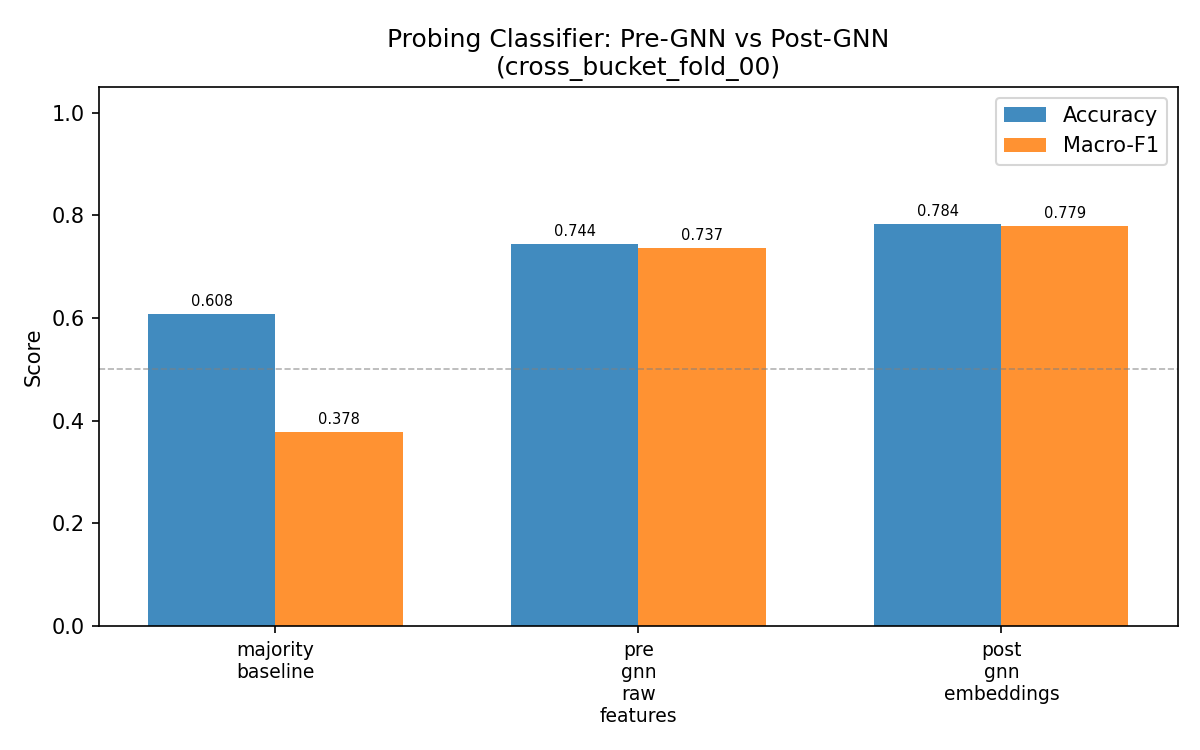
\includegraphics[width=0.65\linewidth]{figures/explainability/probing_bar.png}
  \caption{Probing accuracy at three stages (majority baseline,
  pre-GNN raw features, post-GNN case embedding).  The gap between the
  second and third bars is the \emph{graph's} contribution.}
  \label{fig:probing_bar}
\end{figure}

\paragraph{Result.}
The $+3.97$-point gap between the pre-GNN and post-GNN probe is the
single cleanest measurement of what heterogeneous message passing
contributes on this corpus: identical classifier, identical split,
$16\times$ smaller representation, and still a meaningful accuracy
gain.  In the language of Chapter~\ref{chap:results}, the HGT is
\emph{not} acting as a convoluted text classifier: holding the
downstream head fixed, the graph-propagated representation beats the
text-only representation by a margin that is both statistically and
operationally non-trivial.

\paragraph{What does this embedding space look like?}
Quantifying the gain is necessary but not sufficient.  To see
\emph{how} the representation is reorganised, \path{tsne_visualise.py}
projects pre- and post-GNN embeddings into 2-D with t-SNE, coloured
once by legal-domain bucket and once by outcome label.

\begin{figure}[H]
  \centering
  \begin{minipage}{0.49\textwidth}
    {\footnotesize (a) Pre-GNN, coloured by domain\par}
    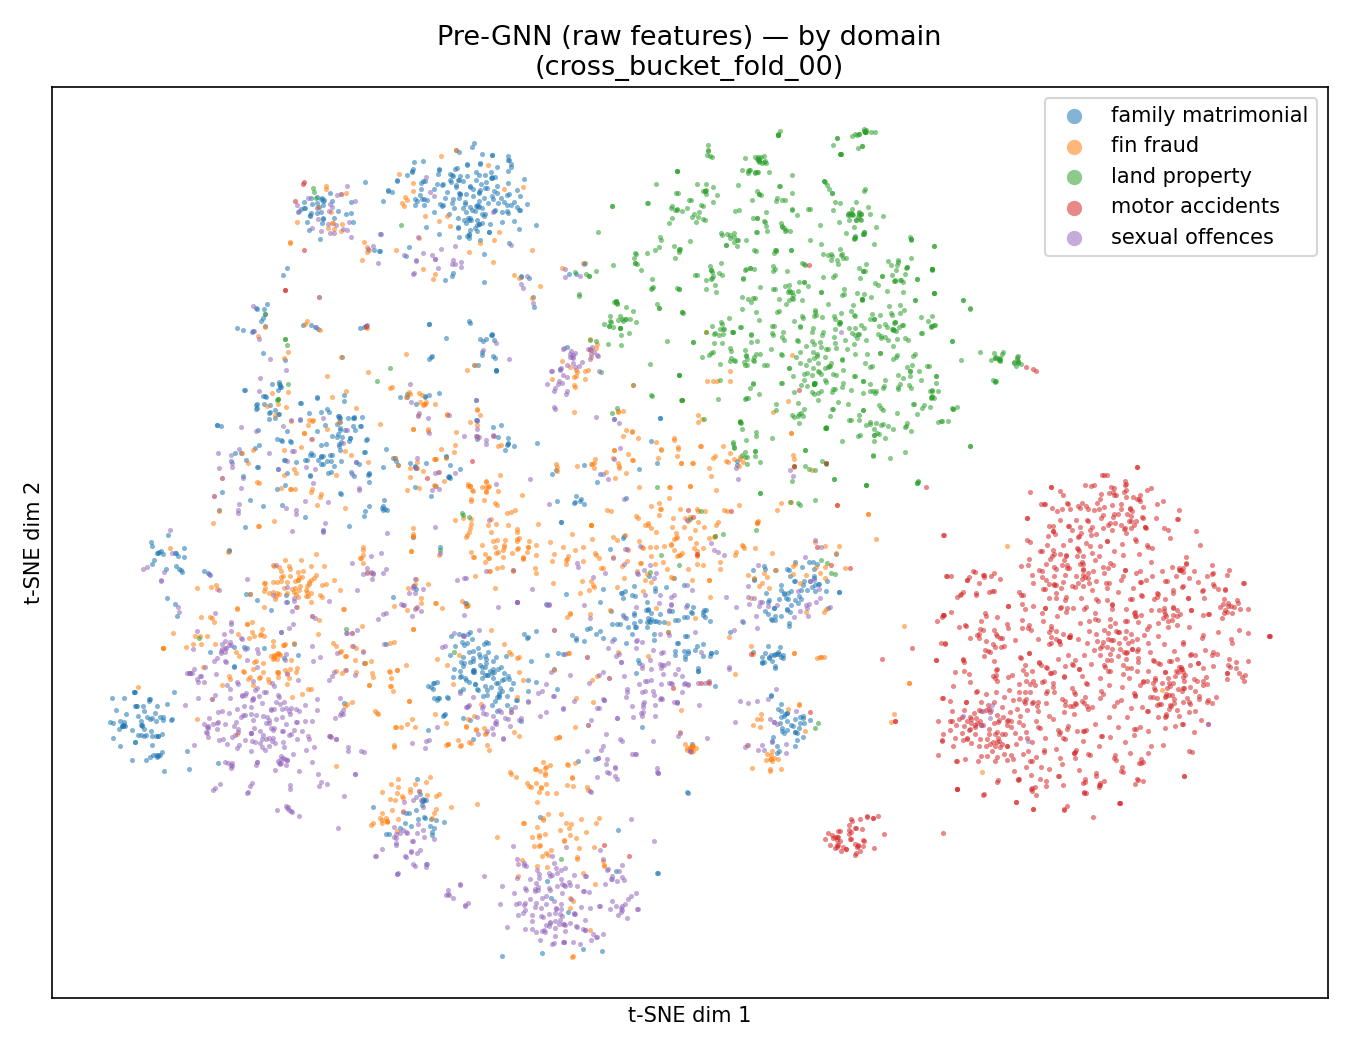
\includegraphics[width=\linewidth]{figures/explainability/tsne_pre_by_domain.png}
  \end{minipage}\hfill
  \begin{minipage}{0.49\textwidth}
    {\footnotesize (b) Post-GNN, coloured by domain\par}
    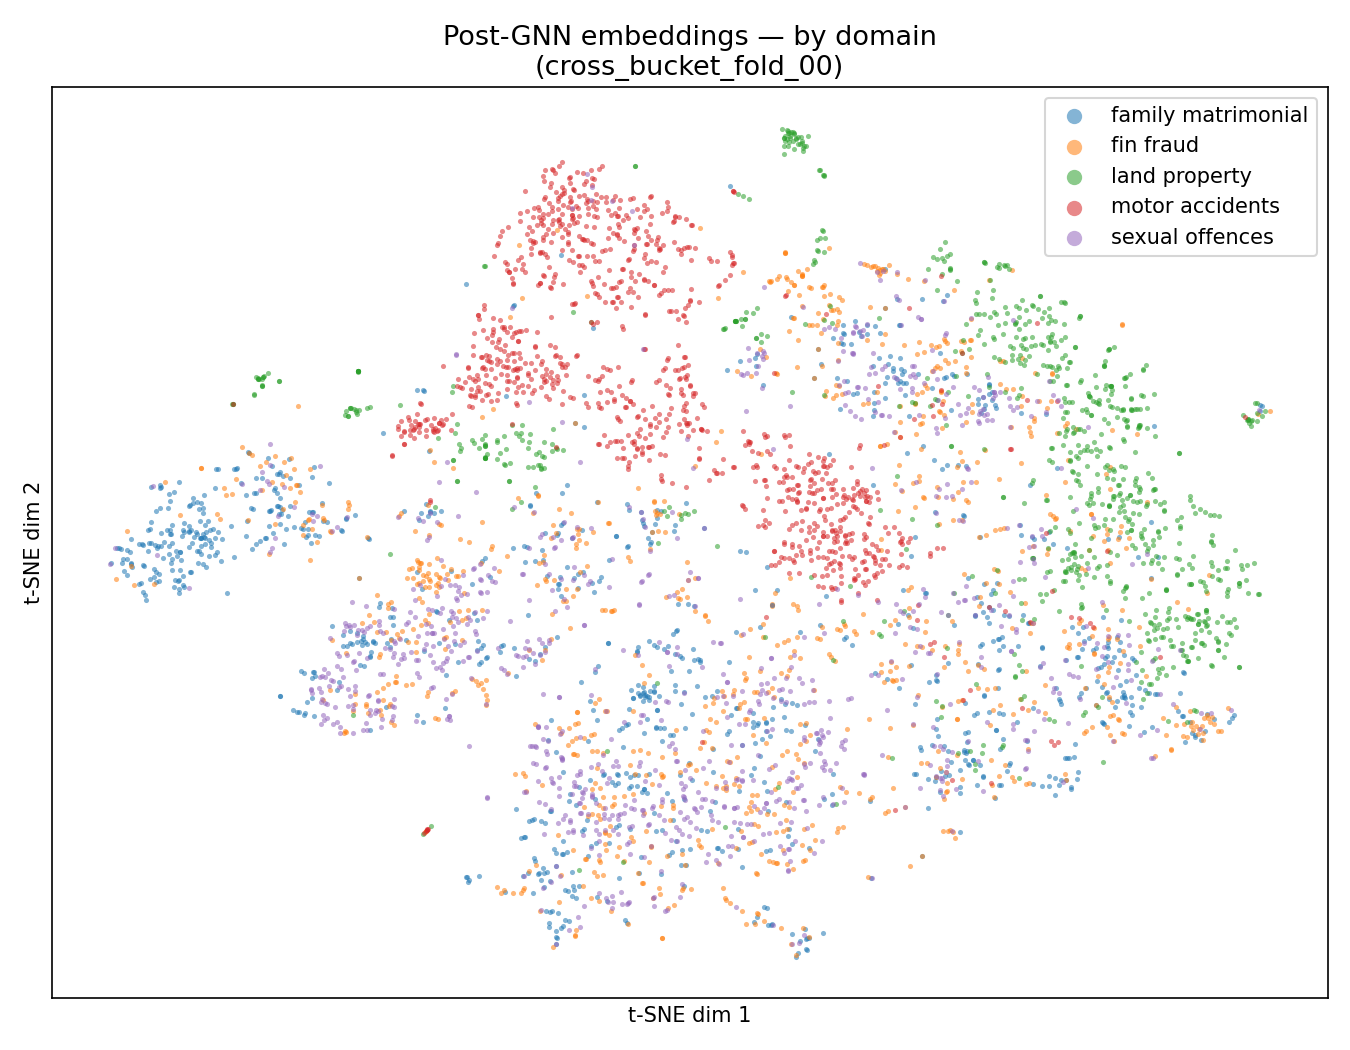
\includegraphics[width=\linewidth]{figures/explainability/tsne_post_by_domain.png}
  \end{minipage}

  \vspace{0.5em}

  \begin{minipage}{0.49\textwidth}
    {\footnotesize (c) Pre-GNN, coloured by outcome label\par}
    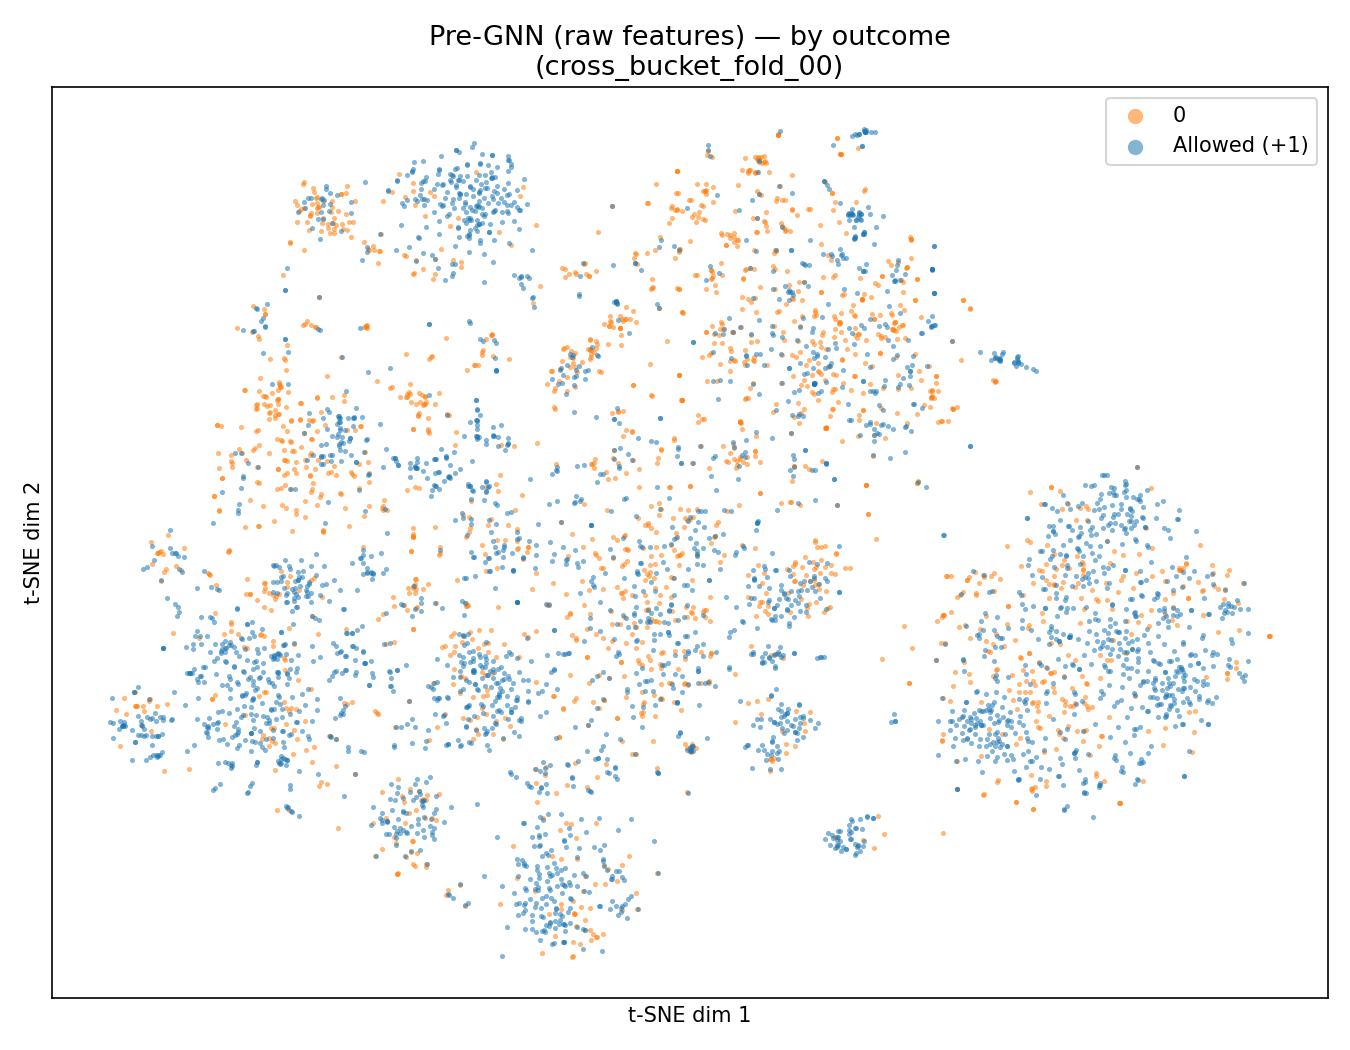
\includegraphics[width=\linewidth]{figures/explainability/tsne_pre_by_label.png}
  \end{minipage}\hfill
  \begin{minipage}{0.49\textwidth}
    {\footnotesize (d) Post-GNN, coloured by outcome label\par}
    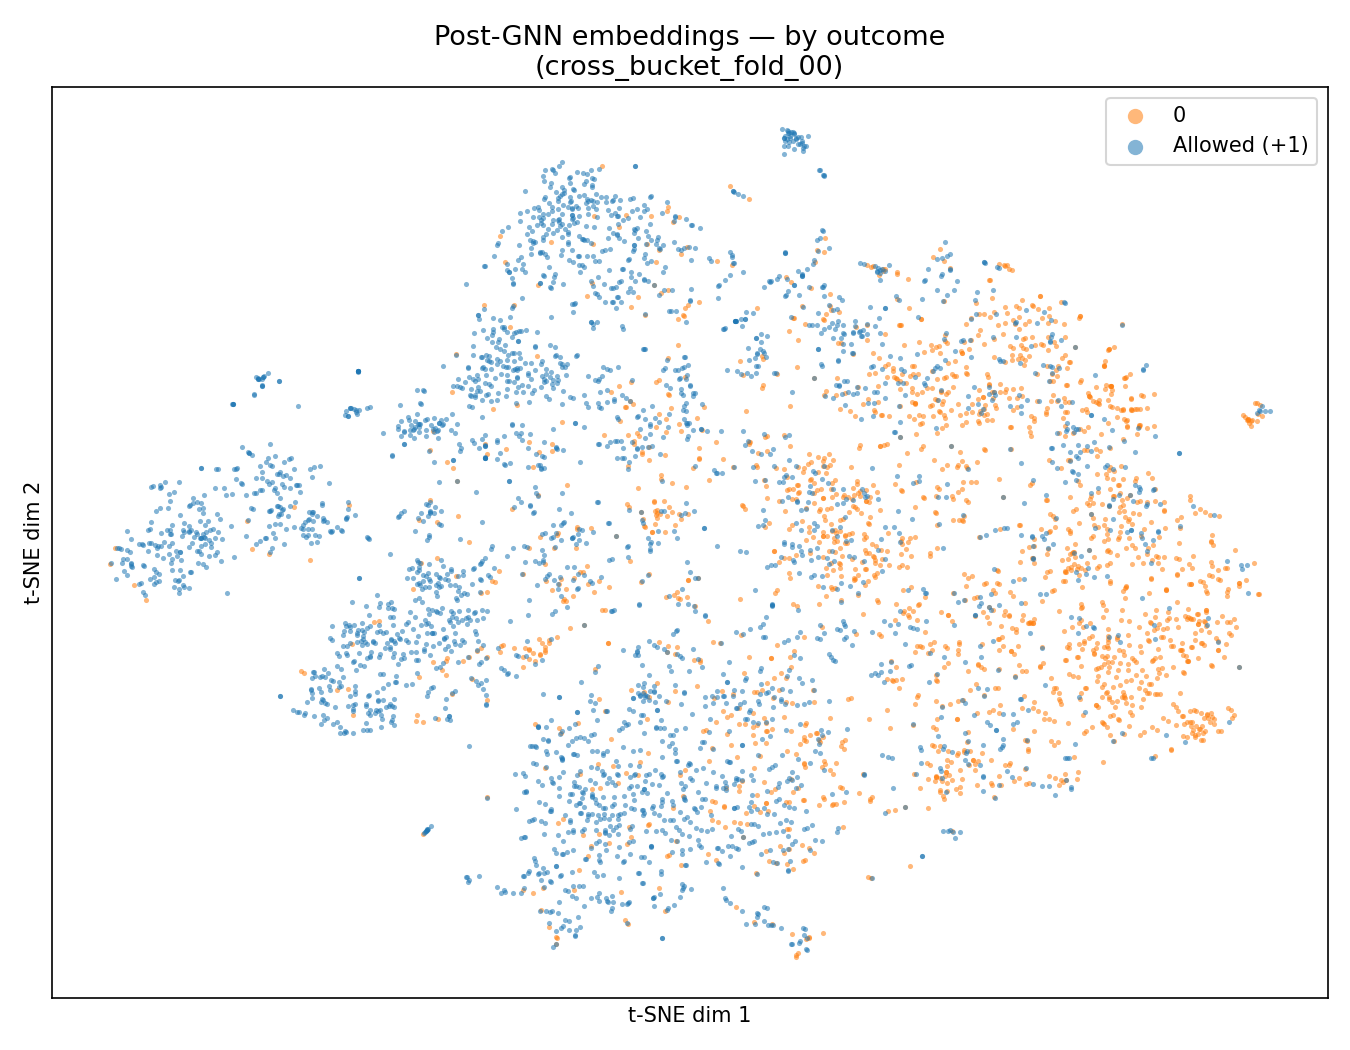
\includegraphics[width=\linewidth]{figures/explainability/tsne_post_by_label.png}
  \end{minipage}
  \caption{t-SNE projections of pre- and post-GNN case embeddings on
  fold~0 of the cross-bucket test split.  Domain structure is already
  present in the pre-GNN view; label structure emerges only after
  graph propagation.}
  \label{fig:repr_tsne}
\end{figure}

The picture is consistent with the probing numbers.  Pre-GNN
embeddings cluster strongly by \emph{domain} --- the \texttt{bge-m3}
representation of the concatenated case text already separates the
five legal buckets --- but outcome labels are mixed within each
cluster.  Post-GNN embeddings preserve the domain clusters but
reorganise each cluster internally so that outcome colour becomes
visibly structured.  The HGT's contribution is therefore primarily
\emph{within-domain} label geometry, not between-domain
reorganisation: message passing uses the shared hubs to sharpen
outcome separation inside each legal neighbourhood.

\section{Component-Level Analysis: Which Parts of the Graph Matter?}
\label{sec:component_analysis}

\paragraph{Problem.}
The representation-level analysis tells us the graph adds signal; it
does not tell us \emph{which} parts of the graph add it.  The
heterogeneous schema has many node types and many edge types, and the
ablation table in Chapter~\ref{chap:results}
(Table~\ref{tab:cross_bucket_results}) shows that removing any one of
them has only a modest effect.  That is a coarse test: it measures
\emph{re-trained} performance without a component.  A complementary
question is, for the \emph{same} frozen model, which components is
the prediction \emph{using} on a case-by-case basis?

\paragraph{Three complementary probes.}
\path{node_importance.py}, \path{attention_analysis.py}, and
\path{shap_analysis.py} answer three different slices of that
question, and using them together reduces the risk of any single
method producing a misleading ranking.

\begin{figure}[H]
  \centering
  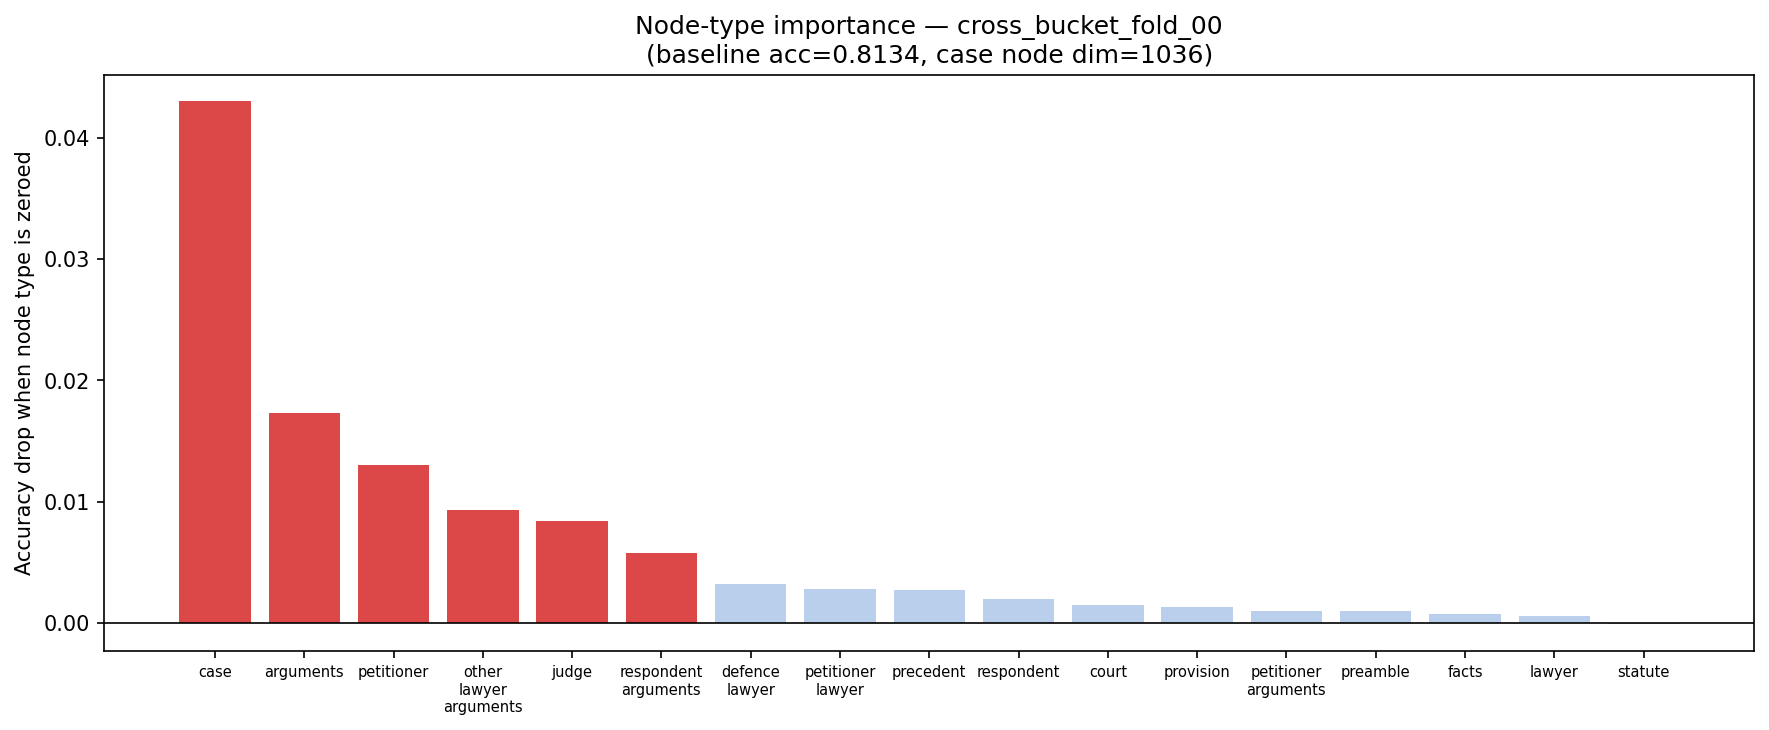
\includegraphics[width=0.78\linewidth]{figures/explainability/node_importance.png}
  \caption{Node-type importance via input zeroing on the cross-bucket
  baseline, fold~0.  Each bar is the accuracy drop when the listed
  node type's features are zeroed before forward pass, holding the
  graph and the remaining features constant.  The \textsc{Case} node
  dominates, followed by the argument-bearing text nodes and the
  \textsc{Petitioner} and \textsc{Judge} participants.}
  \label{fig:node_importance}
\end{figure}

\paragraph{Node-type zeroing.}
For each node type in turn, all features of that type are replaced
with zeros and the frozen HGT is re-evaluated; the drop in test
accuracy is the node type's importance.  Because the graph topology
is preserved, this isolates the \emph{featural} contribution of each
type.  On the cross-bucket baseline (fold~0, baseline accuracy
$0.8134$) the ranking is:
\textsc{Case} ($-0.0430$) $\gg$
\textsc{Arguments} ($-0.0173$) $>$
\textsc{Petitioner} ($-0.0130$) $>$
\textsc{Other\_Lawyer\_Arguments} ($-0.0093$) $>$
\textsc{Judge} ($-0.0084$) $>$
\textsc{Respondent\_Arguments} ($-0.0058$) $>$ remaining types
$\leq\!0.0032$; statute zeroing is within noise of baseline.
Two readings are worth making explicit.  First, the model remains
\emph{anchored in the case node itself}: its own text features are
the dominant source of information, which is consistent with the
architectural choice of reading out from the \textsc{Case} node.
Second, the remaining signal is distributed across the argument
stream and the immediate participants (\textsc{Petitioner},
\textsc{Other\_Lawyer\_Arguments}, \textsc{Judge}) rather than
concentrated on any single authority type --- individual
\textsc{Statute} and \textsc{Provision} nodes have near-zero
per-type importance, so the cross-case signal they carry flows
through the arguments rather than directly through statutory
features.  This supports the claim from Chapter~\ref{chap:results}
that the HGT is not a thinly-disguised text classifier: every
top-tier component is a piece of graph-local legal context that the
\textsc{Case} node aggregates.

\paragraph{Per-relation attention and gradient saliency.}
The second probe operates on edges rather than nodes.
\path{attention_analysis.py} extracts the per-relation attention
priors from each HGT layer and sums per-node-type gradient saliency
with respect to the case logit.

\begin{figure}[H]
  \centering
  \begin{minipage}{0.49\textwidth}
    {\footnotesize (a) Per-relation attention heatmap\par}
    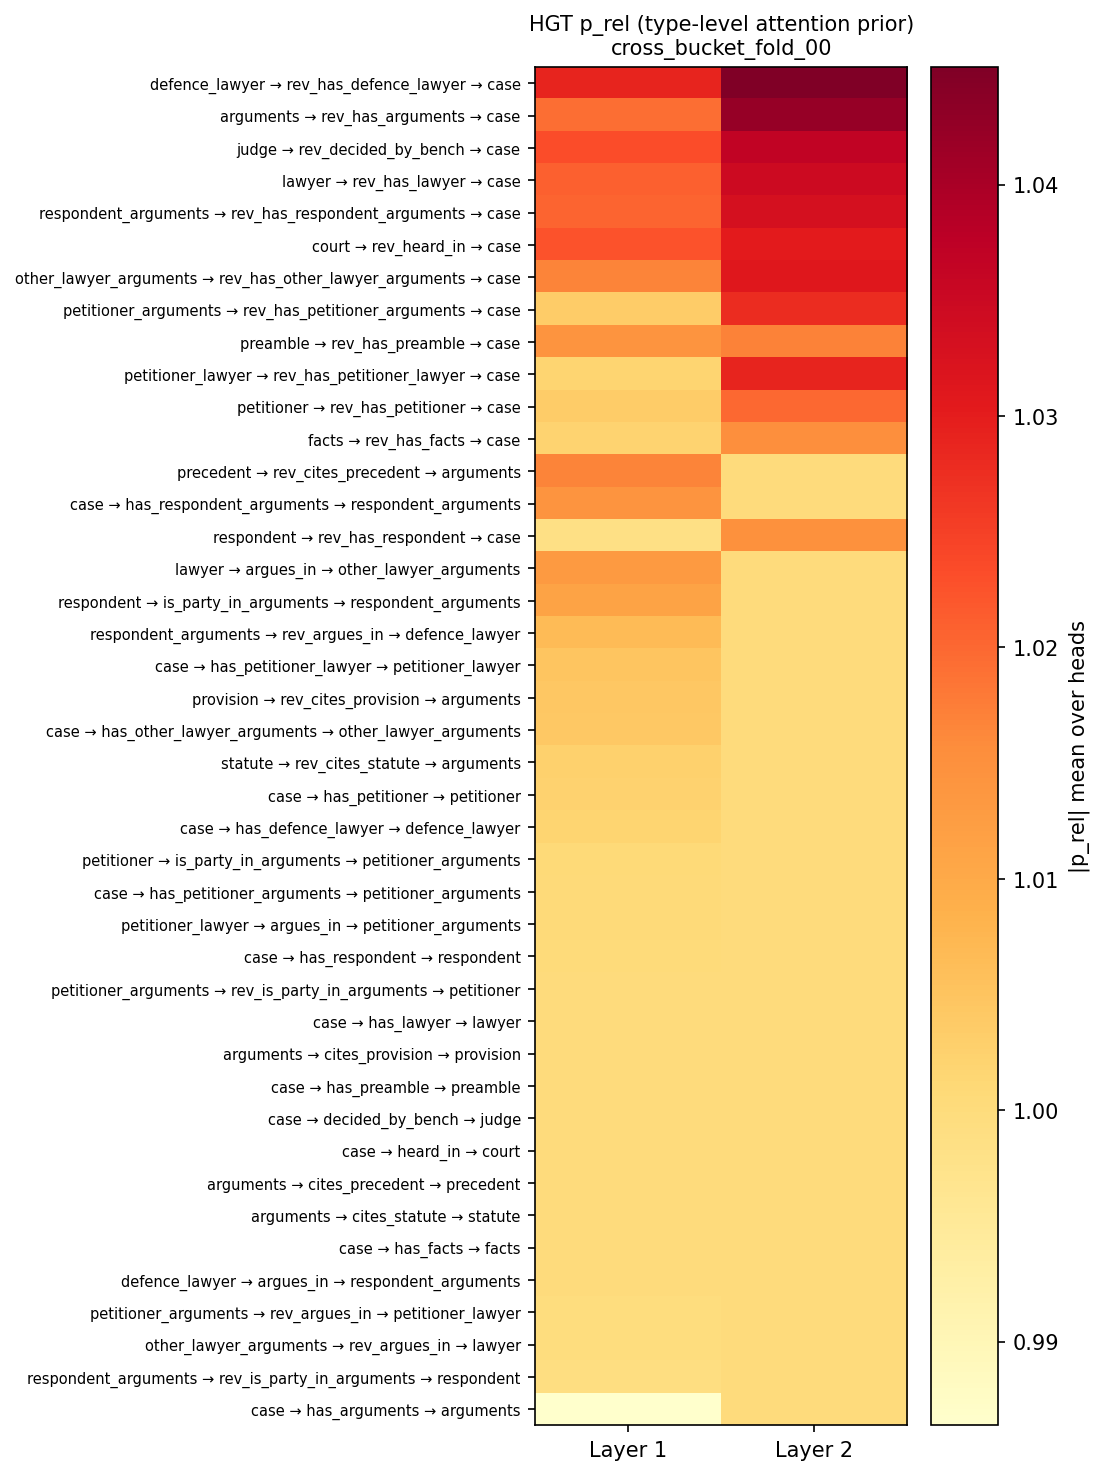
\includegraphics[width=\linewidth]{figures/explainability/prel_heatmap.png}
  \end{minipage}\hfill
  \begin{minipage}{0.49\textwidth}
    {\footnotesize (b) Gradient saliency by node type\par}
    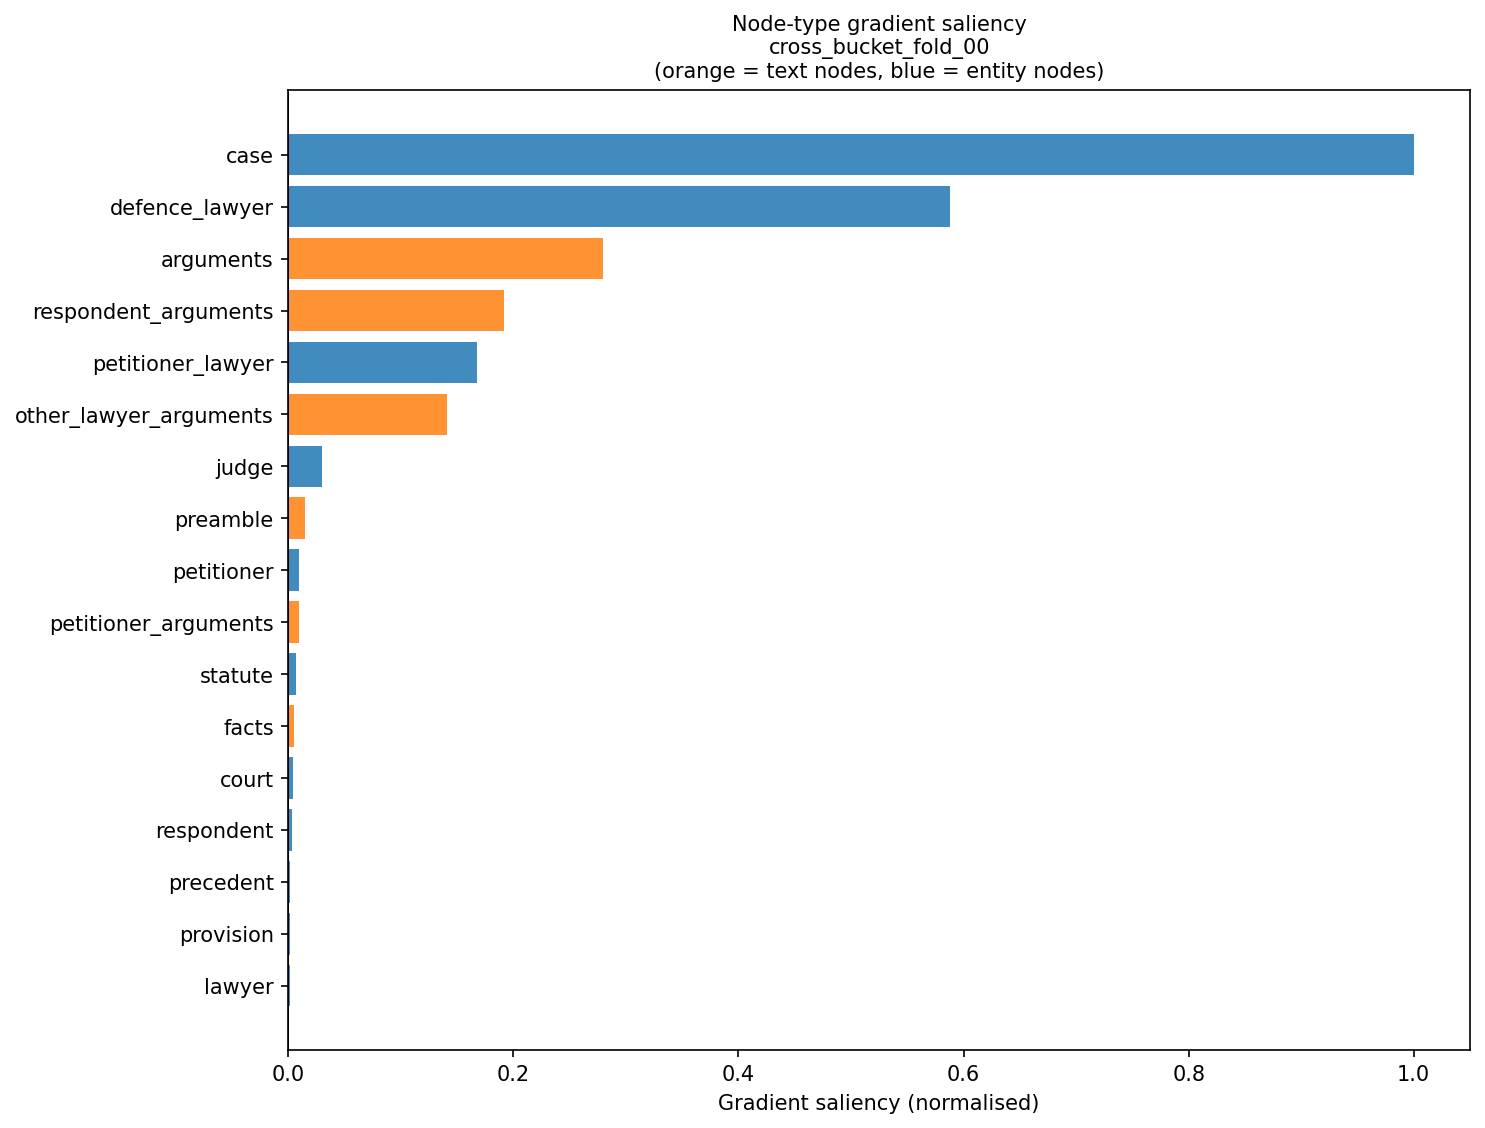
\includegraphics[width=\linewidth]{figures/explainability/gradient_saliency.png}
  \end{minipage}
  \caption{Edge-level attention (a) and node-type gradient saliency
  (b) on the cross-bucket baseline, fold~0.  Reverse edges (those
  delivering information \emph{to} the \textsc{Case} node) dominate
  the attention mass; saliency concentrates on the argument-bearing
  text nodes.}
  \label{fig:attention_saliency}
\end{figure}

Two patterns emerge consistently.  First, the \path{rev_has_*}
edges --- those carrying information \emph{from} text and entity
nodes \emph{back to} the case node --- hold systematically higher
attention mass than their forward counterparts.  This is consistent
with the architecture: the classifier reads only the \textsc{Case}
node's final representation, so a neighbour's value is measured by
how strongly the reverse edge delivers it.  Second, gradient saliency
ranks node types as \textsc{Case} $\gg$ \textsc{Arguments} $>$
\textsc{Other\_Lawyer\_Arguments} $>$ \textsc{Respondent\_Arguments}
$>$ \textsc{Facts} $>$ \textsc{Judge} $>$ \dots, mirroring the
zeroing ranking and confirming that the argument stream is the
operational hinge of the model.

\paragraph{SHAP over the post-GNN embedding.}
The third probe, \path{shap_analysis.py}, computes mean absolute SHAP
values for each dimension of the 64-d post-GNN embedding under a
logistic-regression probe.

\begin{figure}[H]
  \centering
  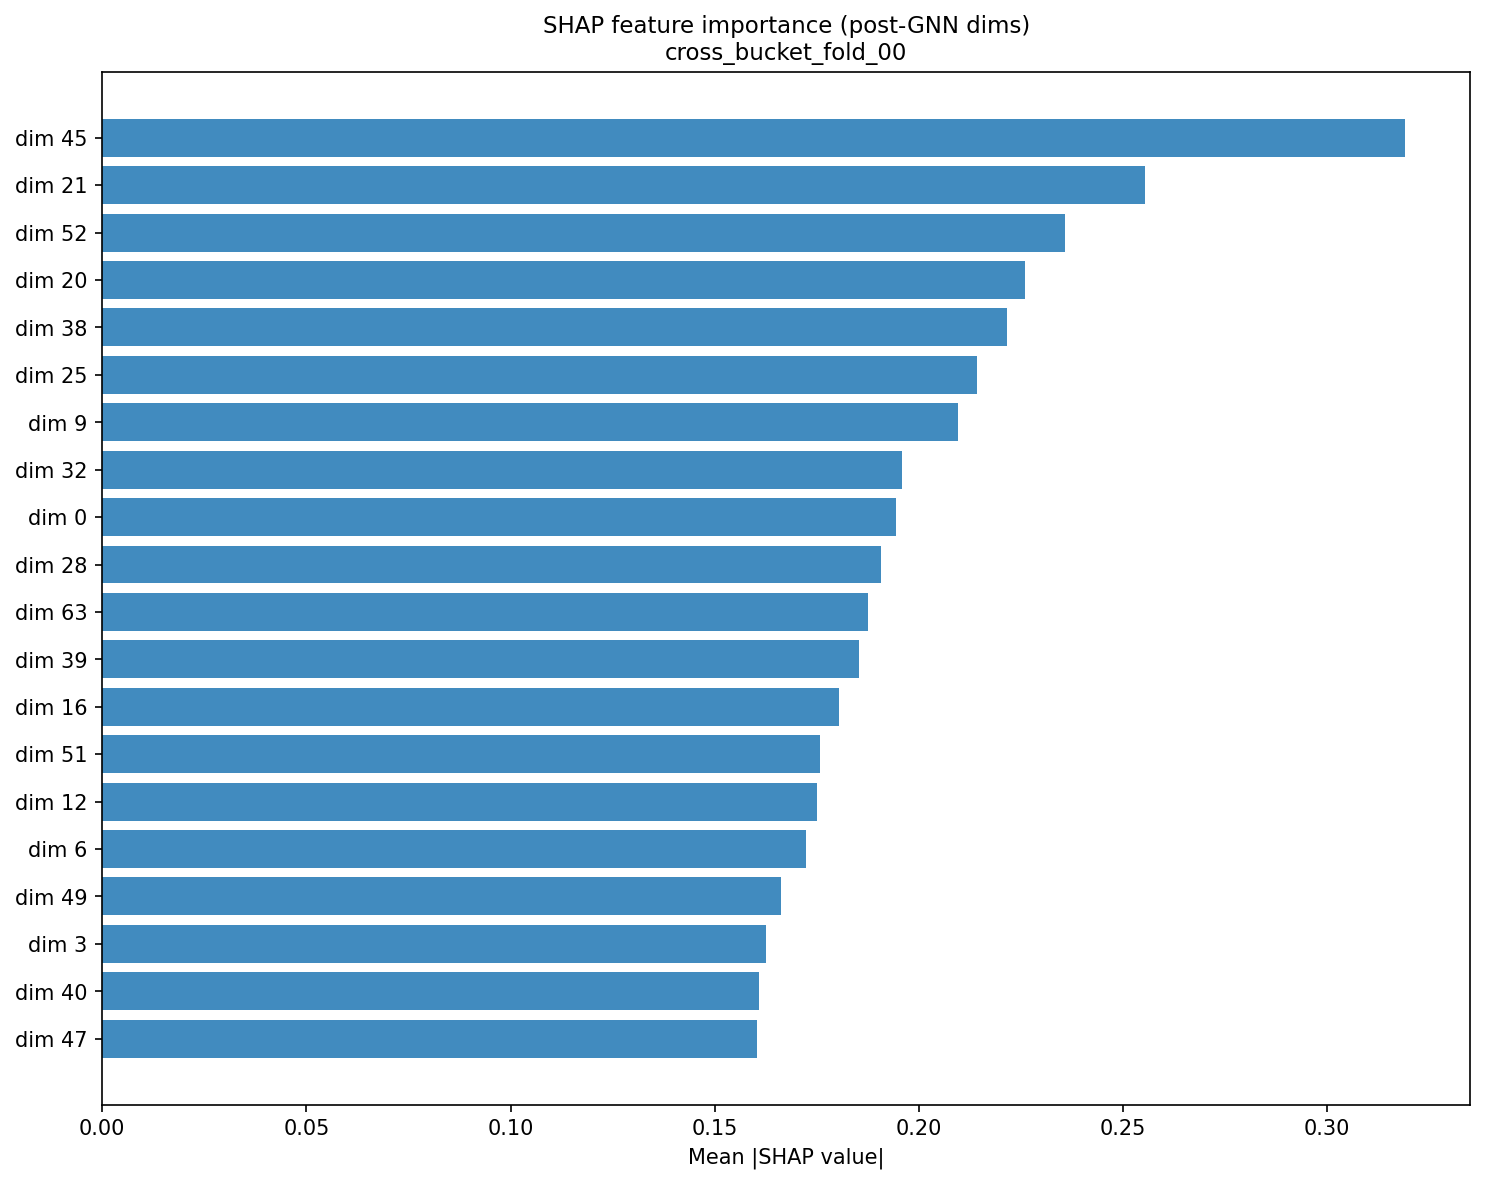
\includegraphics[width=0.78\linewidth]{figures/explainability/shap_bar.png}
  \caption{Mean absolute SHAP values per latent dimension of the
  post-GNN case embedding.  The top six dimensions
  (\texttt{45, 21, 52, 20, 38, 25}) carry the largest marginal
  contribution, but no single dimension dominates.}
  \label{fig:shap_bar}
\end{figure}

No single dimension dominates: the top six dimensions each contribute
meaningfully, but the remaining $58$ dimensions still sum to a
comparable share of the total mass.  A distributed embedding is
exactly what one would want from a graph-level representation ---
collapse onto a small number of dimensions would be evidence of
representational bottleneck.  It is worth stressing, however, that
SHAP operates on the \emph{latent} space: it identifies important
embedding \emph{dimensions}, not interpretable legal concepts.  For
that reason, this probe is used as a \emph{representation diagnostic}
rather than as the final legal explanation; the case-level pipeline
of Section~\ref{sec:case_pipeline} is what produces legally named
evidence.

\section{Error-Level Analysis: Where Does the Representation Fail?}
\label{sec:error_analysis}

\paragraph{Problem.}
Having established that the GNN learns a useful representation and
identified which graph components it depends on, the next
interpretability question is inverse: \emph{where does this
representation stop working?}  The overall test accuracy averages out
failure modes that may be concentrated in identifiable regions of the
data.  Localising them is a prerequisite for knowing when a
prediction can be trusted.

\paragraph{Approach.}
\path{error_analysis.py} decomposes test accuracy along four
orthogonal axes: legal domain, the number of statute nodes attached
to a case (a proxy for doctrinal density), the length of the
\textsc{Facts} section (a proxy for narrative complexity), and the
judgment year (a proxy for temporal drift).

\begin{figure}[H]
  \centering
  \begin{minipage}{0.49\textwidth}
    {\footnotesize (a) Accuracy by legal domain\par}
    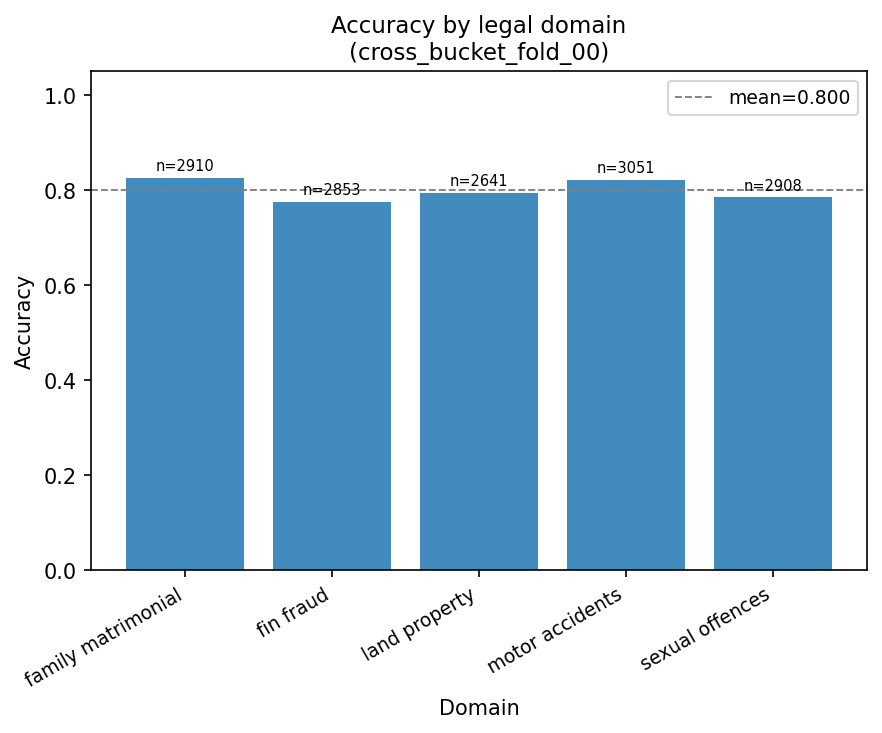
\includegraphics[width=\linewidth]{figures/explainability/error_by_domain.png}
  \end{minipage}\hfill
  \begin{minipage}{0.49\textwidth}
    {\footnotesize (b) Accuracy by judgment year\par}
    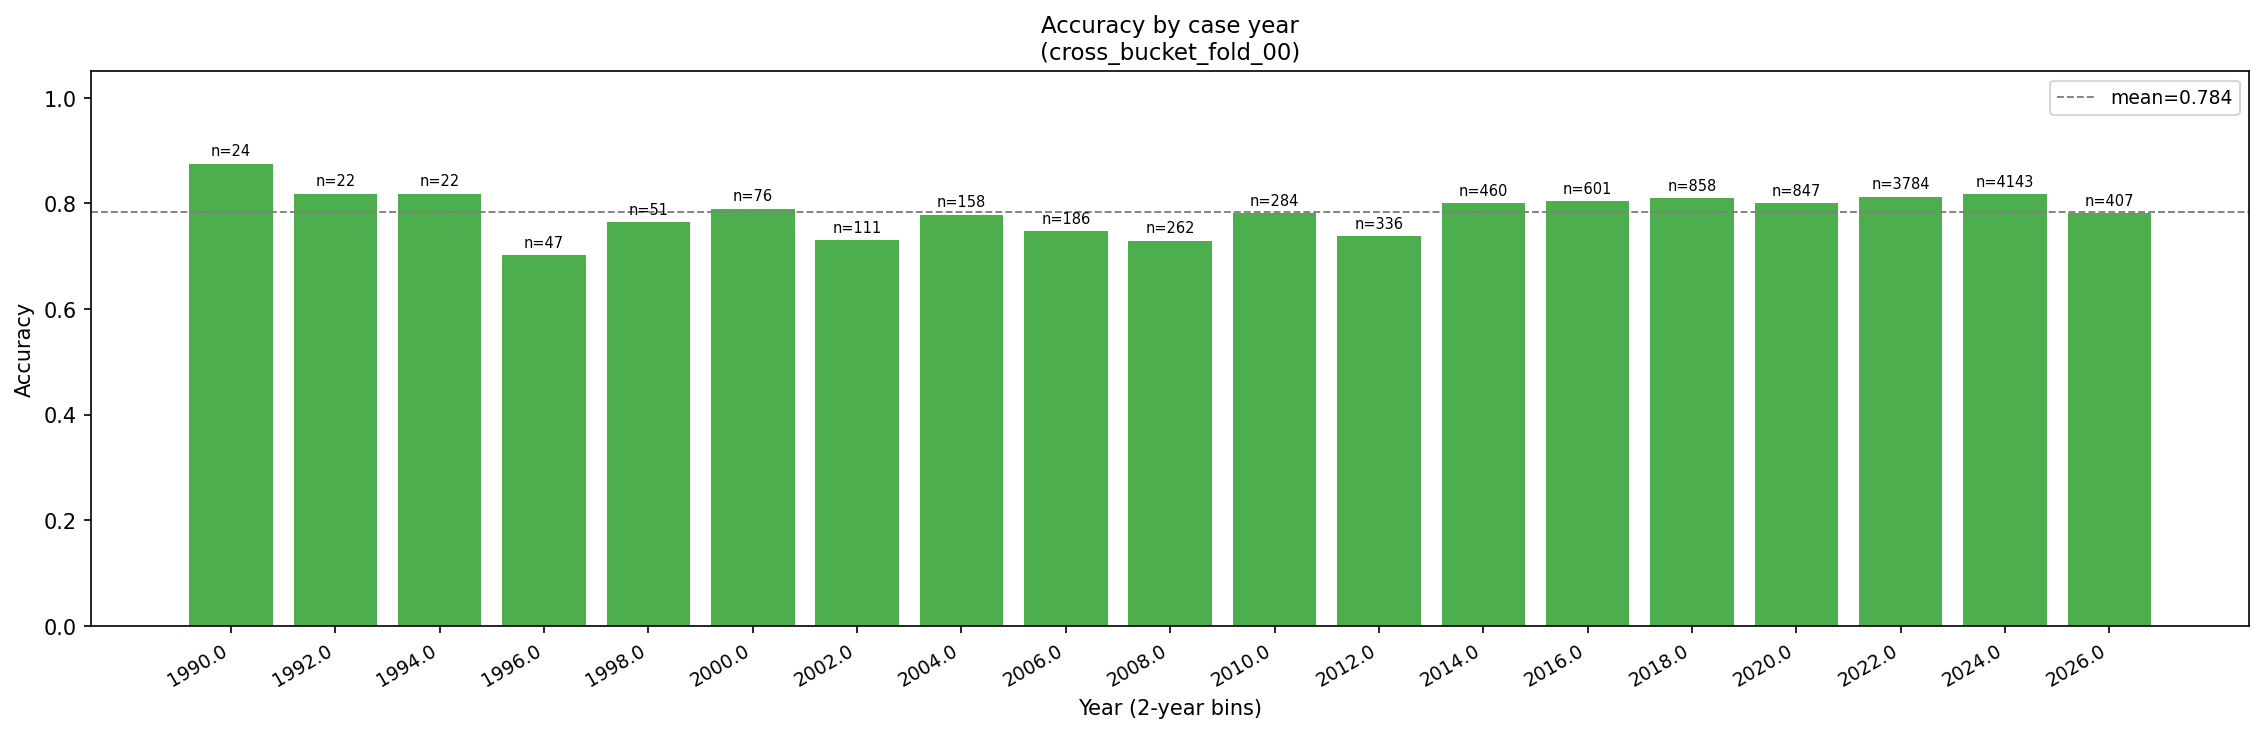
\includegraphics[width=\linewidth]{figures/explainability/error_by_year.png}
  \end{minipage}
  \caption{Error decomposition by legal domain and by year on the
  cross-bucket baseline (fold~0).  Domain ordering is stable across
  ablations; year shows no systematic drift once the small-$n$ early
  years are excluded.}
  \label{fig:error_domain_year}
\end{figure}

\begin{figure}[H]
  \centering
  \begin{minipage}{0.49\textwidth}
    {\footnotesize (a) Accuracy by statute-count bucket\par}
    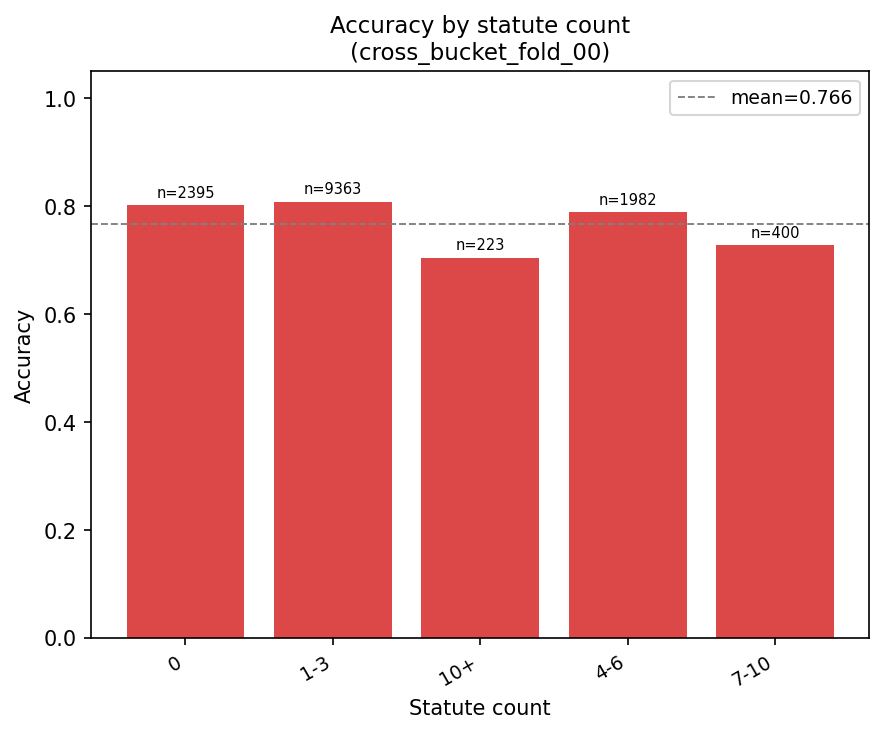
\includegraphics[width=\linewidth]{figures/explainability/error_by_statute.png}
  \end{minipage}\hfill
  \begin{minipage}{0.49\textwidth}
    {\footnotesize (b) Accuracy by facts-length quintile\par}
    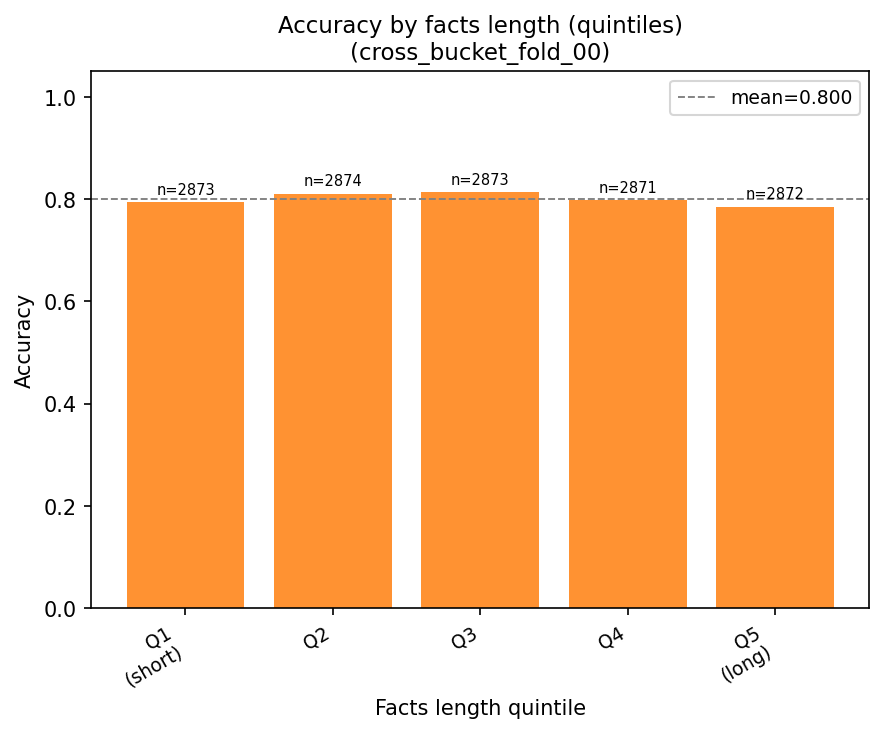
\includegraphics[width=\linewidth]{figures/explainability/error_by_facts_len.png}
  \end{minipage}
  \caption{Error decomposition by doctrinal density (a) and narrative
  complexity (b).  Accuracy falls steadily on cases citing many
  statutes and on cases with the longest facts sections.}
  \label{fig:error_by_structure}
\end{figure}

\paragraph{Findings.}
Several patterns replicate across ablation variants and therefore
look like properties of the data rather than of any specific
configuration.

\begin{itemize}
  \item \textbf{Domain ordering.}  Overall test accuracy is $0.8005$;
    \emph{family~\&~matrimonial} is the strongest domain at $0.8254$,
    \emph{motor~accidents} at $0.8209$; \emph{financial~fraud} at
    $0.7757$ and \emph{sexual~offences} at $0.7844$ are the weakest.
    This ordering tracks structural properties of the buckets
    identified in Chapter~\ref{chap:graph_exploration}: repetitive,
    highly-connected sub-graphs are easier to generalise over than
    the doctrinally heterogeneous fraud and sexual-offence cases.
  \item \textbf{Doctrinal density hurts.}  Accuracy falls from
    $\sim\!0.80$ on cases with 0--3 statute nodes to $0.7040$ on
    cases with $10+$ statute nodes.  The model is fundamentally
    better-behaved in \emph{single-frame} disputes than in
    statutorily crowded judgments where several remedial pathways
    coexist.
  \item \textbf{Long narratives are slightly harder.}  Accuracy on
    the longest-facts quintile is $0.7852$ versus $\sim\!0.81$ on the
    shortest; the decline is modest but monotone.  This is the
    failure pattern that the \texttt{hierarchical\_enc} ablation
    from Chapter~\ref{chap:results} was designed to mitigate, and it
    explains why that ablation helps more on the buckets with long
    \textsc{Arguments} blocks.
  \item \textbf{Year is not a factor.}  After excluding the very
    earliest years (small $n$, non-representative), per-year
    accuracy is flat: no evidence of temporal drift.
\end{itemize}

These failure modes motivate case-level explanation.  The global
probes have now answered the what, which, and where questions.  What
they cannot answer is the \emph{why} for any individual prediction
--- in particular, why a statute-dense case was mis-classified, or
why the confident-wrong predictions reported below all look
structurally plausible to the model.  That question requires a
case-scale pipeline.

\section{Case-Level Explanation}
\label{sec:case_pipeline}

\paragraph{Problem.}
The global analyses above treat the model as a statistical object.
For a specific test case, a legal user needs something different: a
ranked set of \emph{legally named} entities --- statutes, provisions,
precedents, argument spans --- that the frozen model actually relied
on, together with a short list of \emph{analogous training cases}
that sit nearest to it in the model's representation space, and a
natural-language synthesis of both that a practitioner can read.

\paragraph{Approach.}
\path{Graph_Analyser} implements this as a five-phase pipeline over
the frozen HGT checkpoint.  Its bridge to the global analyses is the
post-GNN embedding: Section~\ref{sec:repr_analysis} established that
this embedding encodes outcome-relevant structure, so it is also the
natural basis for retrieval-based case-level explanation.

\begin{table}[H]
  \centering
  \small
  \begin{adjustbox}{max width=\textwidth}
  \begin{tabular}{lll}
    \toprule
    Phase & Script & Primary outputs \\
    \midrule
    1--2: Inference + Index
      & \path{phase1_2_inference_and_index.py}
      & case embeddings, predictions, FAISS index over train split \\
    3: Explainer Training
      & \path{phase3_train_explainer.py}
      & trained heterogeneous PGExplainer \\
    4: Importance Extraction
      & \path{phase4_extract_importance.py}
      & per-case ranked statutes/provisions/precedents/arguments + similar cases \\
    5: LLM Translation
      & \path{phase5_llm_translate.py}
      & grounded natural-language narrative per case \\
    \bottomrule
  \end{tabular}
  \end{adjustbox}
  \caption{The five-phase \texttt{Graph\_Analyser} pipeline.  Phases~1--4
  run in the \texttt{graph\_explainer} environment (PyTorch~2.6,
  PyG~2.7, FAISS); Phase~5 runs in the \texttt{llm} environment
  (vLLM~0.11 serving Mistral-Small~24B).  All phases operate on a
  single frozen checkpoint.}
  \label{tab:explainer_pipeline}
\end{table}

The experiments in this section use the \emph{cross-bucket} pooled
graph, fold~00 of the k-fold split --- 71{,}813 cases total, split
into 51{,}705 training, 5{,}745 validation, and 14{,}363 test ---
with the best-performing checkpoint from
Chapter~\ref{chap:results}, namely the
\texttt{party\_args\_lr\_decay} HGT (hidden dimension 64, two
message-passing layers, four attention heads, dropout $0.25$).
Using the pooled checkpoint rather than a single-domain one is
deliberate: it lets the explainer operate over the full shared hub
structure, so neighbour retrieval and evidence extraction can
cross domain boundaries when the representation says they should.

\subsection{Phase 1--2: Frozen Inference and Retrieval Index}

The first step is to run the frozen HGT in inference mode over the
full graph and collect, for every case node, the 64-d post-GNN
embedding together with the predicted outcome label and its per-class
probabilities.  These are written to \path{case_embeddings.npy} and
\path{predictions.csv}.

Retrieval-based explanation requires an index that answers
``\emph{which training cases are nearest to this test case in the
model's representation space?}''  Phase~2 builds a FAISS cosine
similarity index (\path{train_faiss.index}, \path{train_indices.npy})
over the training-split embeddings only.  Using cosine distance on
the post-GNN embedding (rather than on raw text features or on an
earlier layer) is a deliberate choice: neighbours returned by this
index are similar \emph{in the sense that matters for the frozen
model's prediction}, not merely similar in input text.  Retrieval and
prediction therefore share a single representation, which is what
makes a retrieved neighbour a legitimate explanatory analogue rather
than a surface-lookup match.

\subsection{Phase 3: Training a Heterogeneous Edge Masker}

The textbook approach to edge attribution on GNNs is PGExplainer
\cite{luo2020parameterized}: a small MLP scores each edge, and the
subset of highest-scoring edges, fed back through the original model,
is required to preserve the prediction.  PyG's implementation is,
however, \emph{homogeneous}: it weights messages via
\texttt{edge\_weight}, which HGTConv does not accept.  Its attention
is defined over typed neighbourhoods, not over scalar-weighted
messages.

\paragraph{Heterogeneous adaptation.}
\path{analyser/hetero_pg_explainer.py} keeps the PGExplainer objective but
changes the mask semantics: instead of weighting messages, the
explainer selects which edges \emph{exist}.  Given a binary edge mask
produced by a shared MLP that ingests source-node embeddings,
destination-node embeddings, and a learnable relation-type embedding,
Phase~3 removes the masked edges from \texttt{edge\_index\_dict} and
reruns the frozen HGT on the reduced graph.  The mask is relaxed to
$[0,1]$ via Gumbel-sigmoid straight-through estimation, which keeps
edge selection discrete at inference time while retaining
differentiability for training.  Training minimises three terms:

\begin{enumerate}
  \item \textbf{Prediction loss.}  Cross-entropy between the frozen
    HGT's predictions on the masked graph and on the full graph.
    Drives the mask to preserve the model's output.
  \item \textbf{Size regulariser.}  An $\ell_1$ penalty on the
    fraction of selected edges; encourages sparse explanations.
  \item \textbf{Entropy regulariser.}  An entropy penalty on the
    edge-score distribution; prevents the explainer from converging
    to uniform weights and forces hard decisions.
\end{enumerate}

Temperature is annealed from $5$ to $1$ over 30 epochs, giving the
optimiser soft exploration early and hard selection at convergence.

\subsection{Phase 4: From Edge Scores to Legal Evidence}

An edge-level importance score is not yet a legal explanation.
Phase~4 translates the trained masker's output into entity-level
answers.  To amortise work across the many test cases being
explained, edge importance is computed once, globally, rather than
per-case: the trained explainer's edge-score function is evaluated on
every edge of the full graph, and each case-level explanation is
assembled by reading off the scores for the edges reachable from the
target case.

For each test case to be explained:

\begin{enumerate}
  \item The $k$-hop subgraph centred on the target case node is
    collected by undirected BFS, with depth matching the HGT's two
    message-passing layers (so the subgraph covers exactly the nodes
    whose information the frozen model could have propagated to the
    case representation).
  \item Edge importance scores from the pre-computed global table
    are restricted to edges incident to the reachable node set.  The
    frozen HGT is \emph{not} re-run per-case: the trained explainer
    is the authoritative source of edge importance for this pipeline.
  \item Edge scores are aggregated to node importance by the
    max-incident-edge rule (a node inherits the maximum score among
    the edges touching it in the reachable subgraph), and nodes are
    ranked by type, producing separate top-$N$ lists for
    \textsc{Statute}, \textsc{Provision}, \textsc{Precedent}, and
    the four argument-node variants.
  \item The Phase~2 FAISS index is queried with the target case's
    post-GNN embedding to retrieve the top-$k$ most similar training
    cases ($k\!=\!3$ by default), together with their labels and a
    compact argument-context snippet.
\end{enumerate}

Each case's output is a JSON record containing predicted and true
labels, confidence scores, ranked entity lists, retrieved neighbour
cases, and the raw numerical evidence that backs each claim.

\subsection{Phase 5: LLM Translation}

The Phase~4 record is machine-readable but not
\emph{human-readable}: a ranked list of node identifiers is not, on
its own, a legal explanation, which requires synthesising the
statutes with the provisions, the provisions with the case facts, and
the case facts with the analogous cases into a coherent narrative.
Phase~5 feeds the Phase~4 record into a Mistral-Small~24B model run
locally under vLLM, with a prompt that asks it to produce a
structured narrative covering the predicted outcome, the governing
statutes, the key provisions, the retrieved analogous precedents, the
argument patterns from the similar training cases, and a plain-language
reasoning summary.

\paragraph{Role boundary.}
The LLM is not used as an open-ended legal reasoner: it receives
\emph{only} the evidence bundle extracted by the frozen model, plus
the pre-outcome textual content of the target case (preamble and
arguments).  The prompt does surface the true outcome as an
\emph{``actual outcome (for reference)''} field alongside the
predicted one so that the generated narrative can flag model errors
rather than silently rationalise them, but the LLM is explicitly
instructed to explain the \emph{predicted} label and is not asked to
re-decide the case.  Its role is verbalisation and synthesis over a
fixed evidence set, not additional prediction.  This boundary ---
evidence selection is done by the trained explainer, verbalisation
by the LLM --- is what makes the resulting narrative attributable to
the HGT's behaviour rather than to LLM priors.

\section{A Worked Example: A Confidently-Correct Case}
\label{sec:worked_correct}

To illustrate the pipeline end-to-end, consider test case~10212
(\emph{Sanjeev Kumar vs State of Punjab and Another}, 19 April 2023).
The frozen HGT predicts \emph{petitioner wins} with probability
$0.9998$; the ground-truth label is also \emph{petitioner wins}.
This is the kind of prediction where a global accuracy number gives
no information about whether the model got the case right for the
right reasons.

\begin{figure}[H]
  \centering
  \begin{minipage}{0.49\textwidth}
    {\footnotesize (a) Target case in post-GNN t-SNE space\par}
    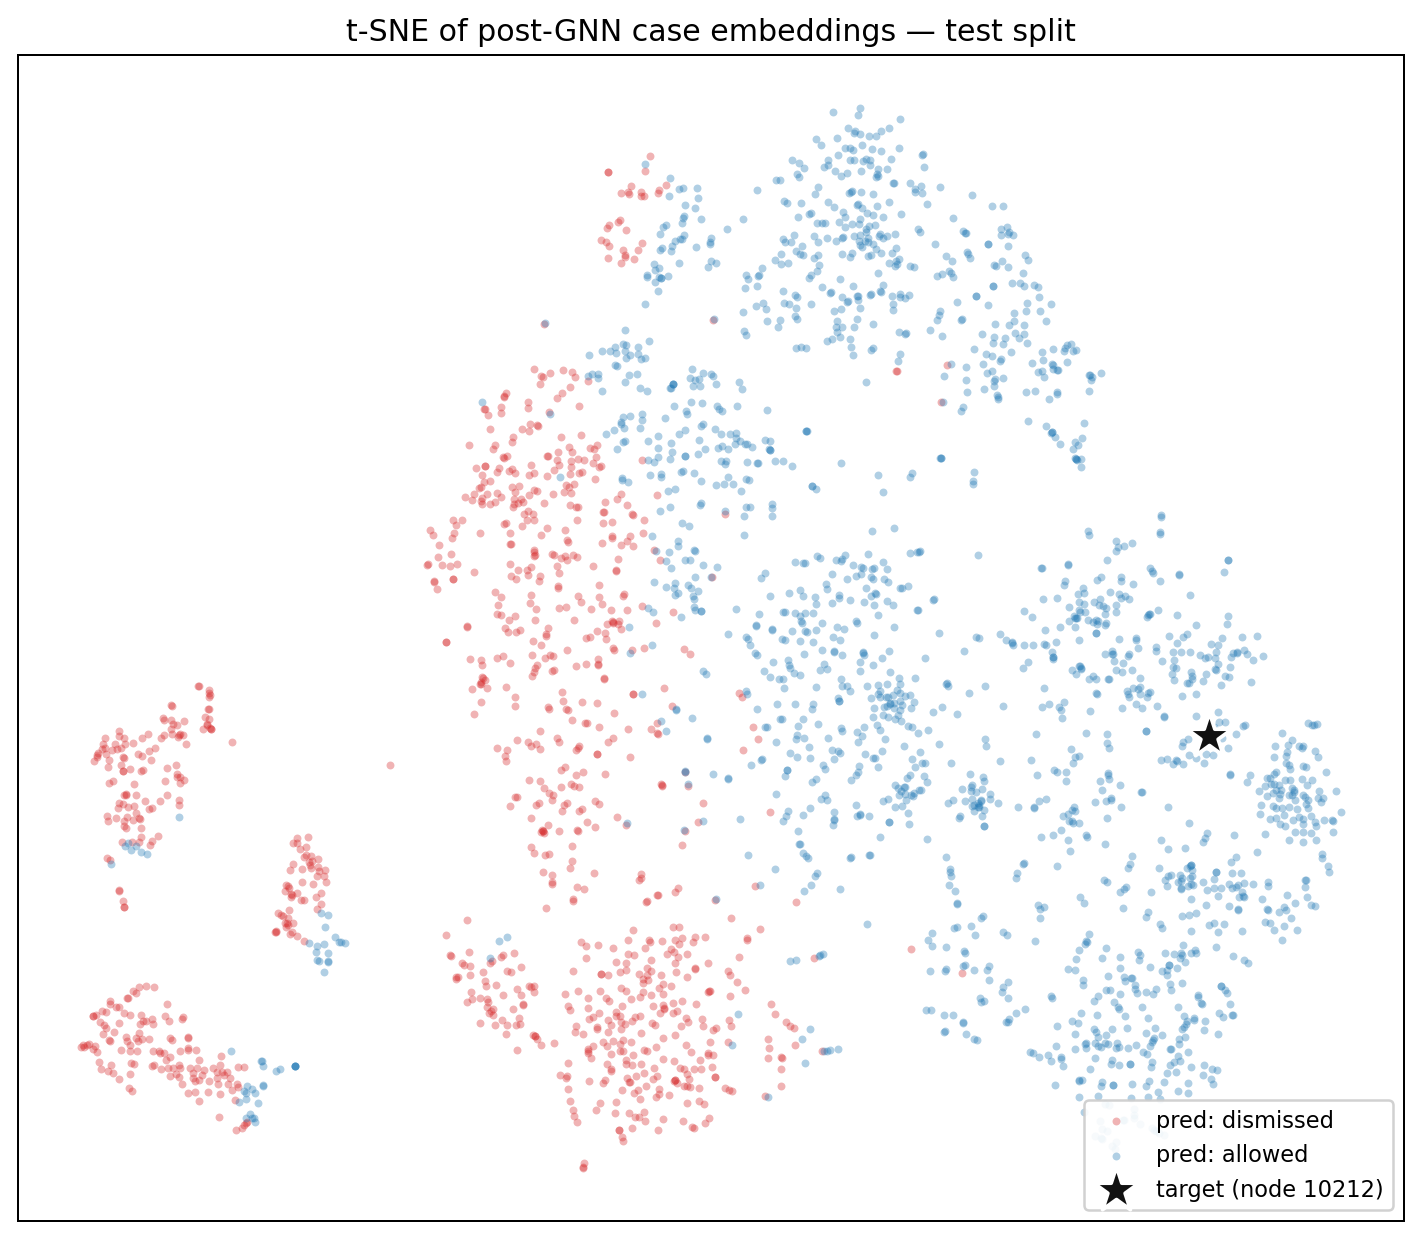
\includegraphics[width=\linewidth]{figures/explainability/correct_10212_panel_a_tsne.png}
  \end{minipage}\hfill
  \begin{minipage}{0.49\textwidth}
    {\footnotesize (b) Top evidence subgraph from the PGExplainer\par}
    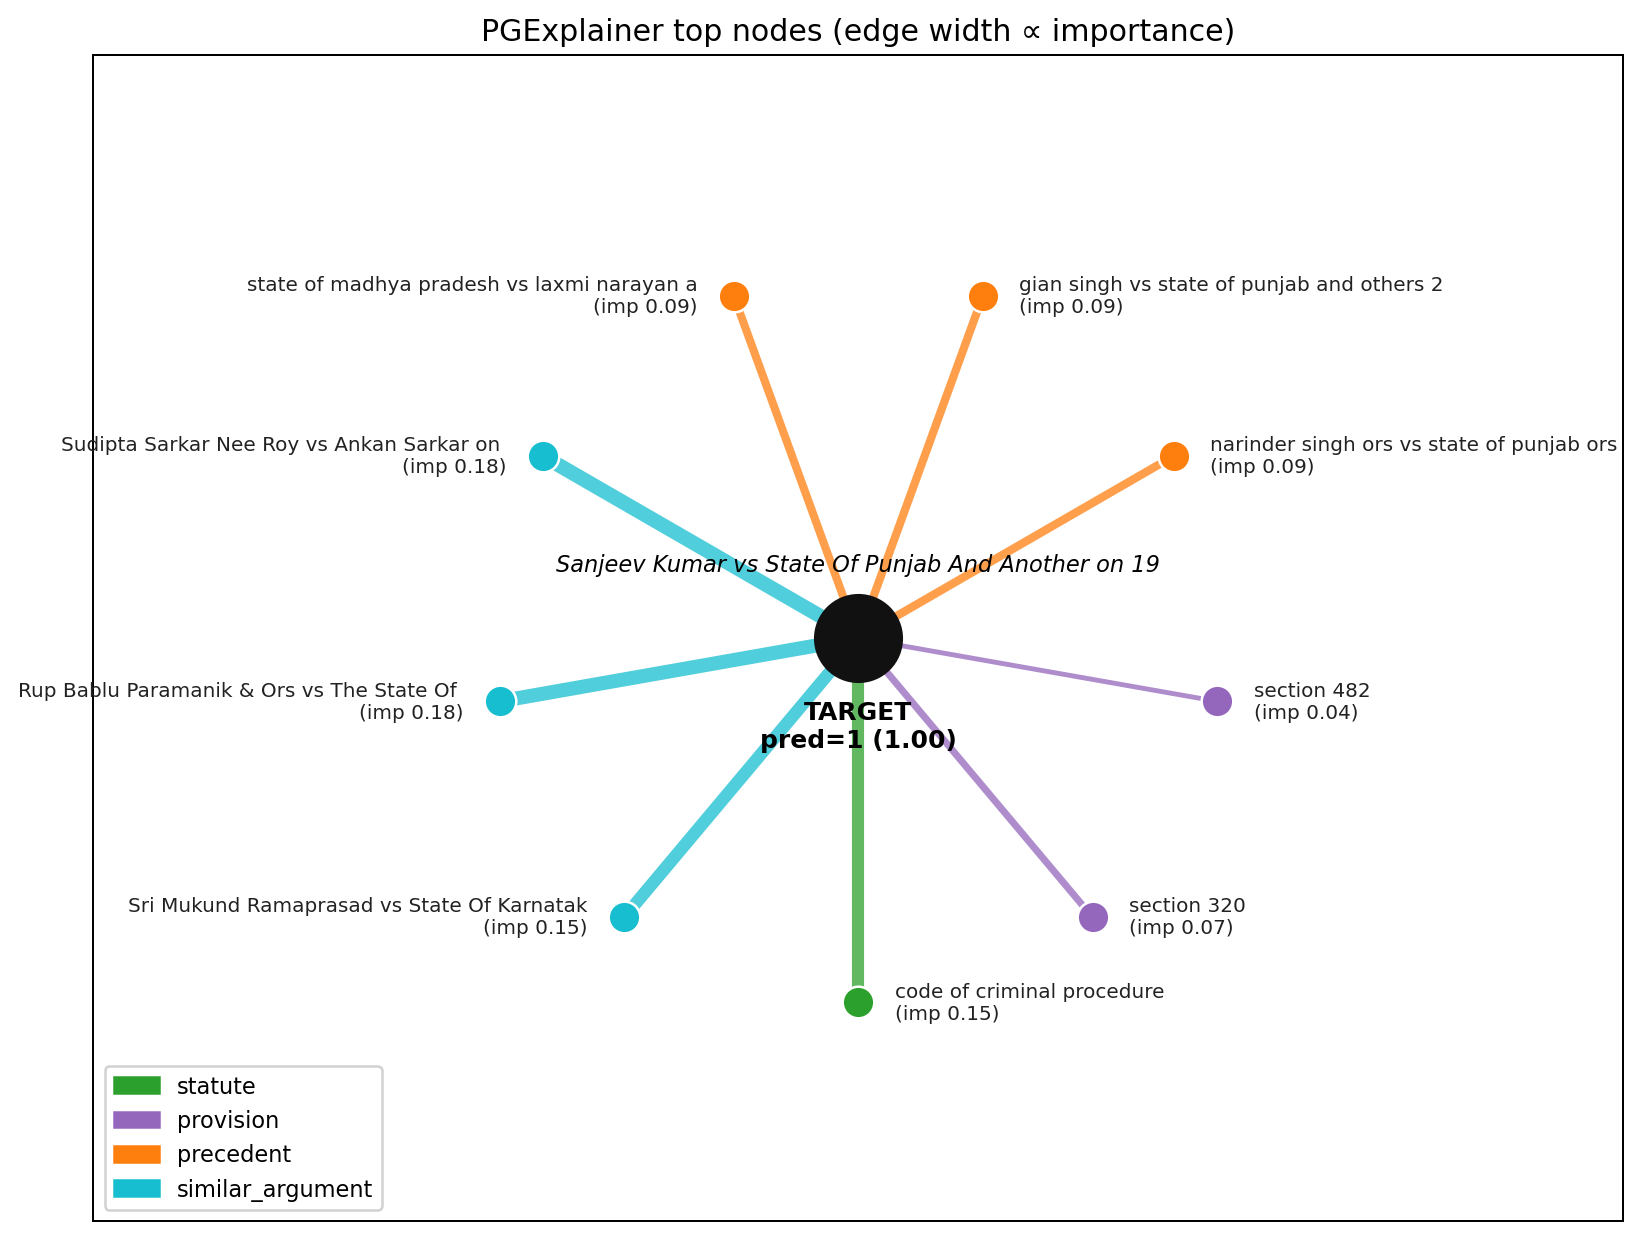
\includegraphics[width=\linewidth]{figures/explainability/correct_10212_panel_b_subgraph.png}
  \end{minipage}
  \caption{Confidently-correct case 10212 (\emph{Sanjeev Kumar vs
  State of Punjab and Another}, 2023).  Panel (a) locates the case in
  post-GNN embedding space; panel (b) shows the top-weighted
  statutes, provisions, precedents, and argument nodes selected by
  the trained edge masker.}
  \label{fig:case_correct}
\end{figure}

\paragraph{Evidence extracted.}
The governing statute surfaced by the masker is the \emph{Code of
Criminal Procedure}.  The top two provisions are Section~320 CrPC
(compounding of offences) and Section~482 CrPC (inherent power of
the High Court to quash proceedings) --- exactly the doctrinal pair
that underlies the family-matrimonial ``quash-on-compromise''
pattern.  The top retrieved analogous training cases are
\emph{Gurmail Singh And Ors vs State of Punjab And Another} (allowed),
\emph{Satinder Pal Verma And Others vs State of Punjab} (allowed),
and \emph{Ravi Kumar Prashar And Anr vs State of Punjab And Another}
(allowed), all with cosine similarity $>\!0.99$ in post-GNN space.

\paragraph{LLM-translated narrative.}
The Phase~5 narrative reconstructs this as standard
quash-on-compromise reasoning: the parties have settled the dispute;
Section~320 CrPC governs compounding; Section~482 CrPC authorises
the High Court to quash proceedings to prevent abuse of process;
\emph{Gian Singh vs State of Punjab} (2012) and \emph{State of MP vs
Laxmi Narayan} (2019) establish that inherent-power quashing is
available even for non-compoundable offences when the compromise is
genuine; the predicted-win outcome therefore aligns with the pattern
of the retrieved neighbours.  This is not the LLM inventing a legal
argument: every named statute, provision, and precedent in the
narrative comes from the Phase~4 evidence bundle, and the analogies
are drawn from the FAISS-retrieved training cases.  What the LLM
supplies is the connective tissue between those pieces.

\section{When Confidence and Correctness Diverge: Structural Error
Analysis}
\label{sec:right_vs_wrong}

The interesting failures of a prediction model are not the
low-confidence mistakes --- those are honest and already reflected in
the calibration --- but the \emph{high-confidence} mistakes.  The
retrieval-based framing of
Section~\ref{sec:case_pipeline} provides a natural diagnostic tool
for them: compare the predicted-class label of the target case's
top-$k$ retrieved neighbours with its true label.

\paragraph{Aggregate statistic.}
\path{confident_wrong_analysis.py} applies this diagnostic to every
test case whose predicted-class probability exceeds $0.99$.
1{,}460 cases are \emph{confidently correct}; $72$ are
\emph{confidently wrong}.  For the confidently wrong subset, the mean
fraction of top-$5$ neighbours matching the \emph{predicted}
(incorrect) label is $0.989$; the mean fraction matching the
\emph{true} label is $0.011$.  $68$ of the $72$ confidently-wrong
cases have all five top neighbours drawn from the predicted class.

\begin{figure}[H]
  \centering
  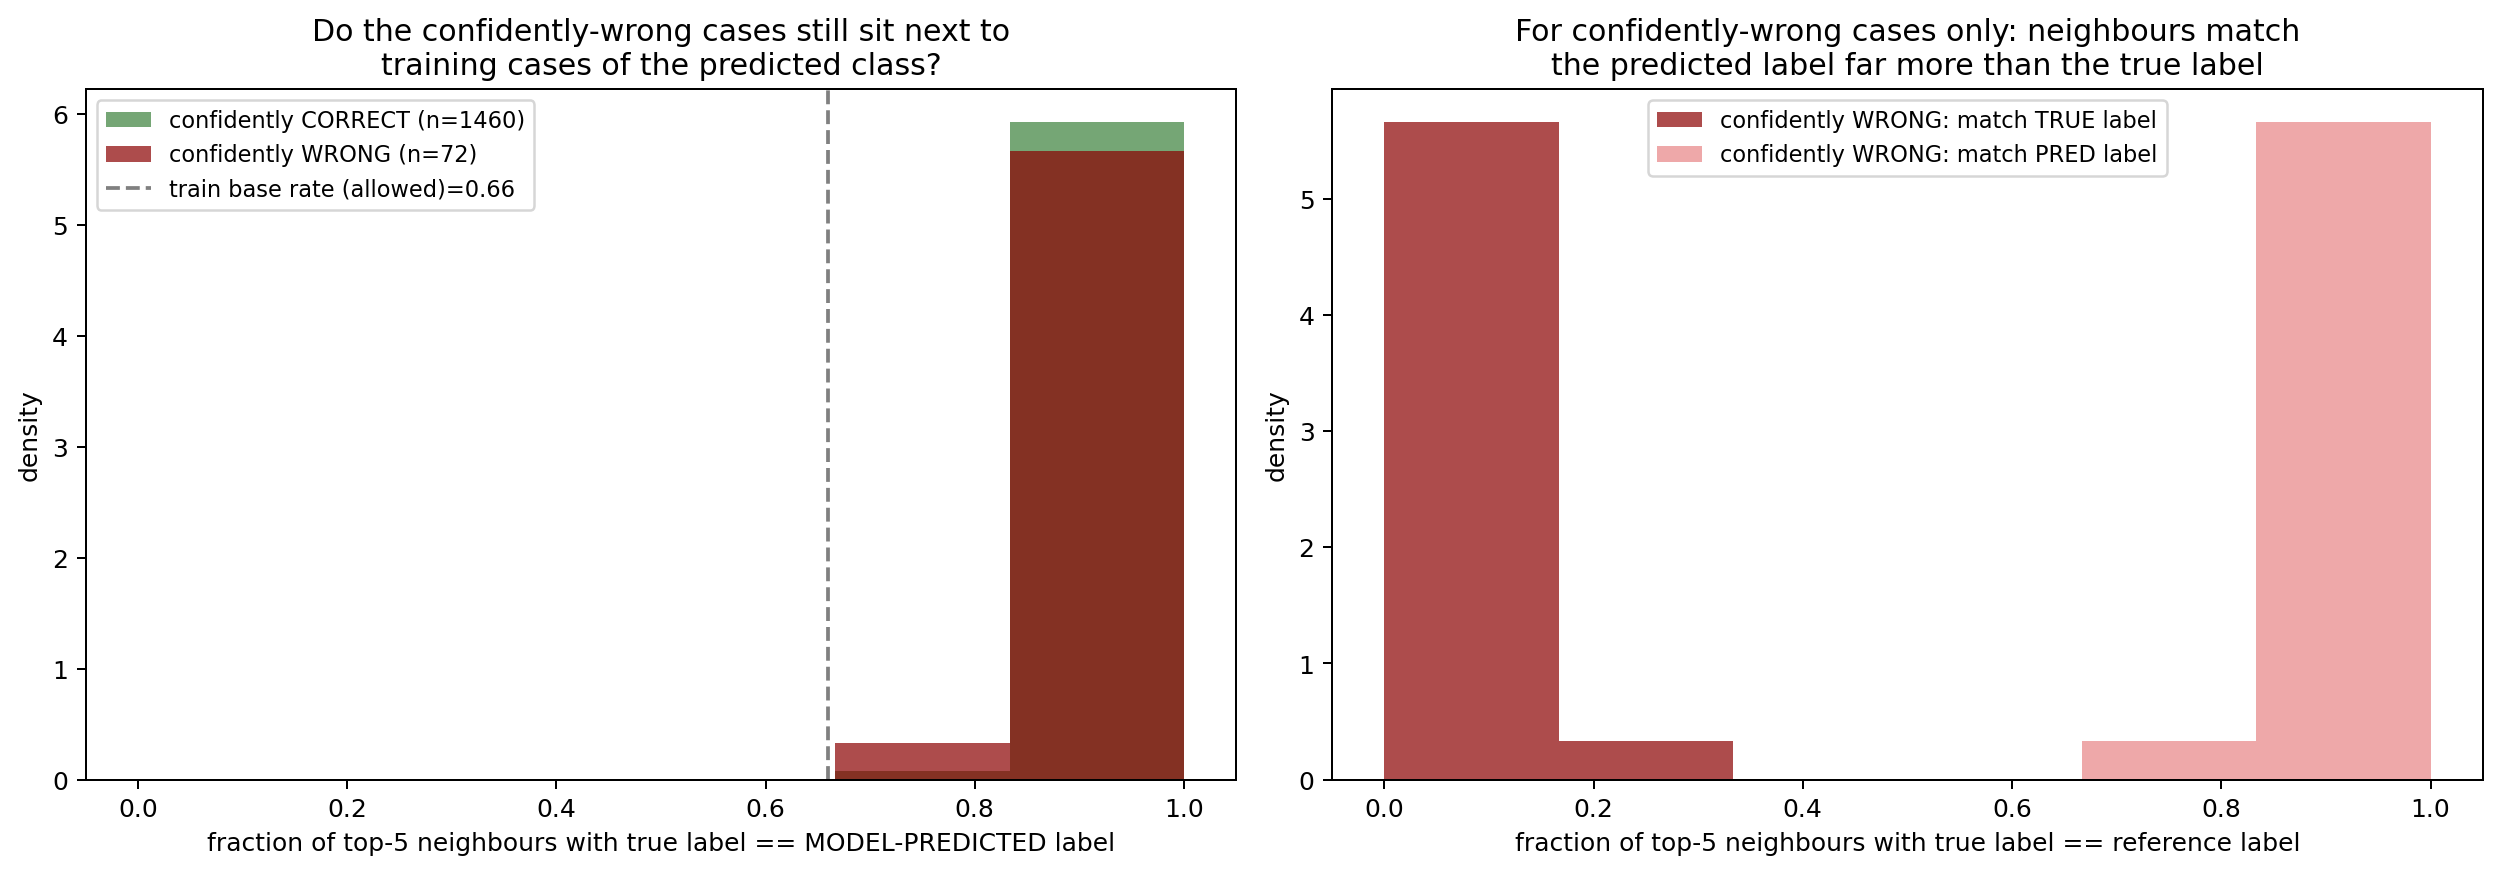
\includegraphics[width=0.78\linewidth]{figures/explainability/neighbour_alignment_hist.png}
  \caption{Distribution of neighbour-label alignment for
  high-confidence predictions.  For confidently-correct cases
  (blue) the top-$5$ neighbours almost always match the true label;
  for confidently-wrong cases (red) they almost always match the
  \emph{predicted} label and disagree with the truth.}
  \label{fig:neighbour_alignment}
\end{figure}

\paragraph{Interpretation.}
Confident errors are not random.  They occur when the post-GNN
embedding places the target case inside the wrong outcome
neighbourhood, causing \emph{both} the prediction and the
retrieval-based explanation to reinforce the same mistaken structure.
This is a sharper failure mode than ``the model is uncertain''.  It
means that the very mechanism used to explain successes ---
representation-space similarity to training cases --- also amplifies
the confident errors, because the retrieved analogues all look like
the class the model wrongly predicts.  Practically, this is an
argument for pairing the prediction with a \emph{class-boundary
proximity} score at deployment time, rather than with classifier
confidence alone.

\paragraph{A worked confident-wrong example.}
Test case 13701 (\emph{Umesh V vs State of Kerala}, 18 January 2023)
is predicted \emph{petitioner wins} with probability $0.9998$; the
true label is \emph{petitioner loses}.  All three displayed
neighbours --- \emph{Faisal P.C.}, \emph{Nisamudheen M.M.}, and
\emph{Nithin Antony} vs \emph{State of Kerala}, filed on the same or
adjacent day --- are wins, each with cosine similarity $>\!0.98$;
the same pattern holds at the $k\!=\!5$ neighbourhood used by the
aggregate confident-wrong analysis above.

\begin{figure}[H]
  \centering
  \begin{minipage}{0.49\textwidth}
    {\footnotesize (a) Target case in post-GNN t-SNE space\par}
    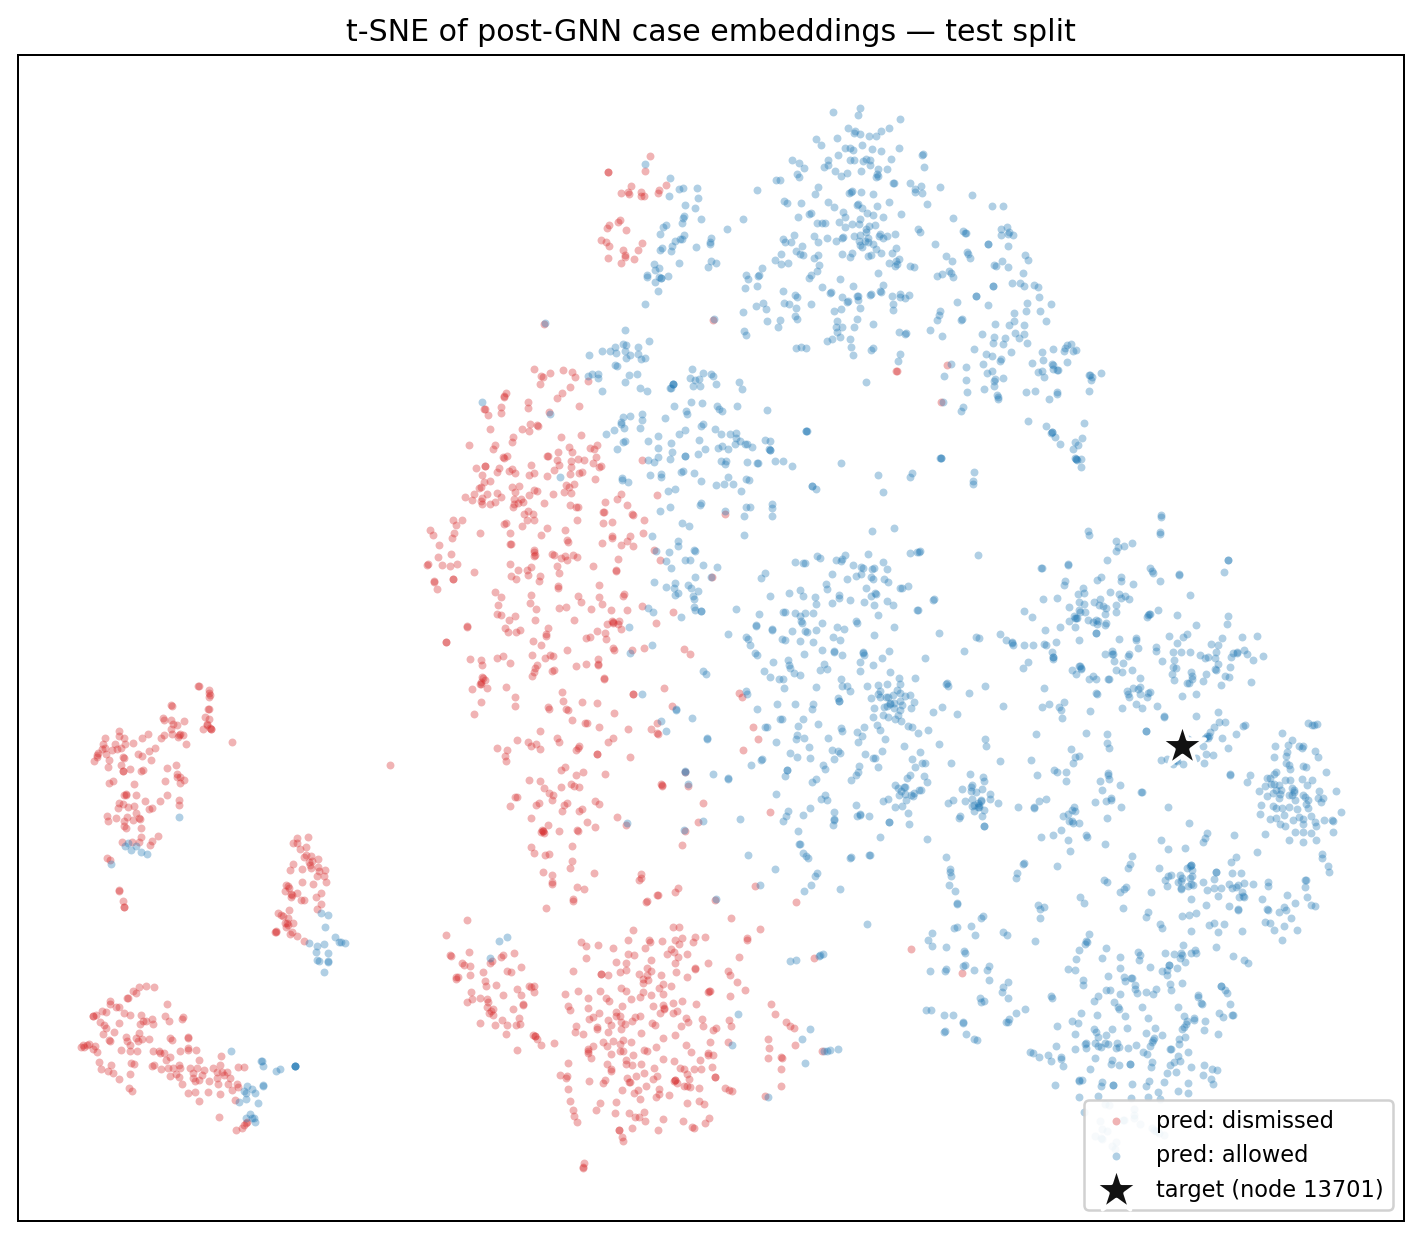
\includegraphics[width=\linewidth]{figures/explainability/wrong_13701_panel_a_tsne.png}
  \end{minipage}\hfill
  \begin{minipage}{0.49\textwidth}
    {\footnotesize (b) Top evidence subgraph\par}
    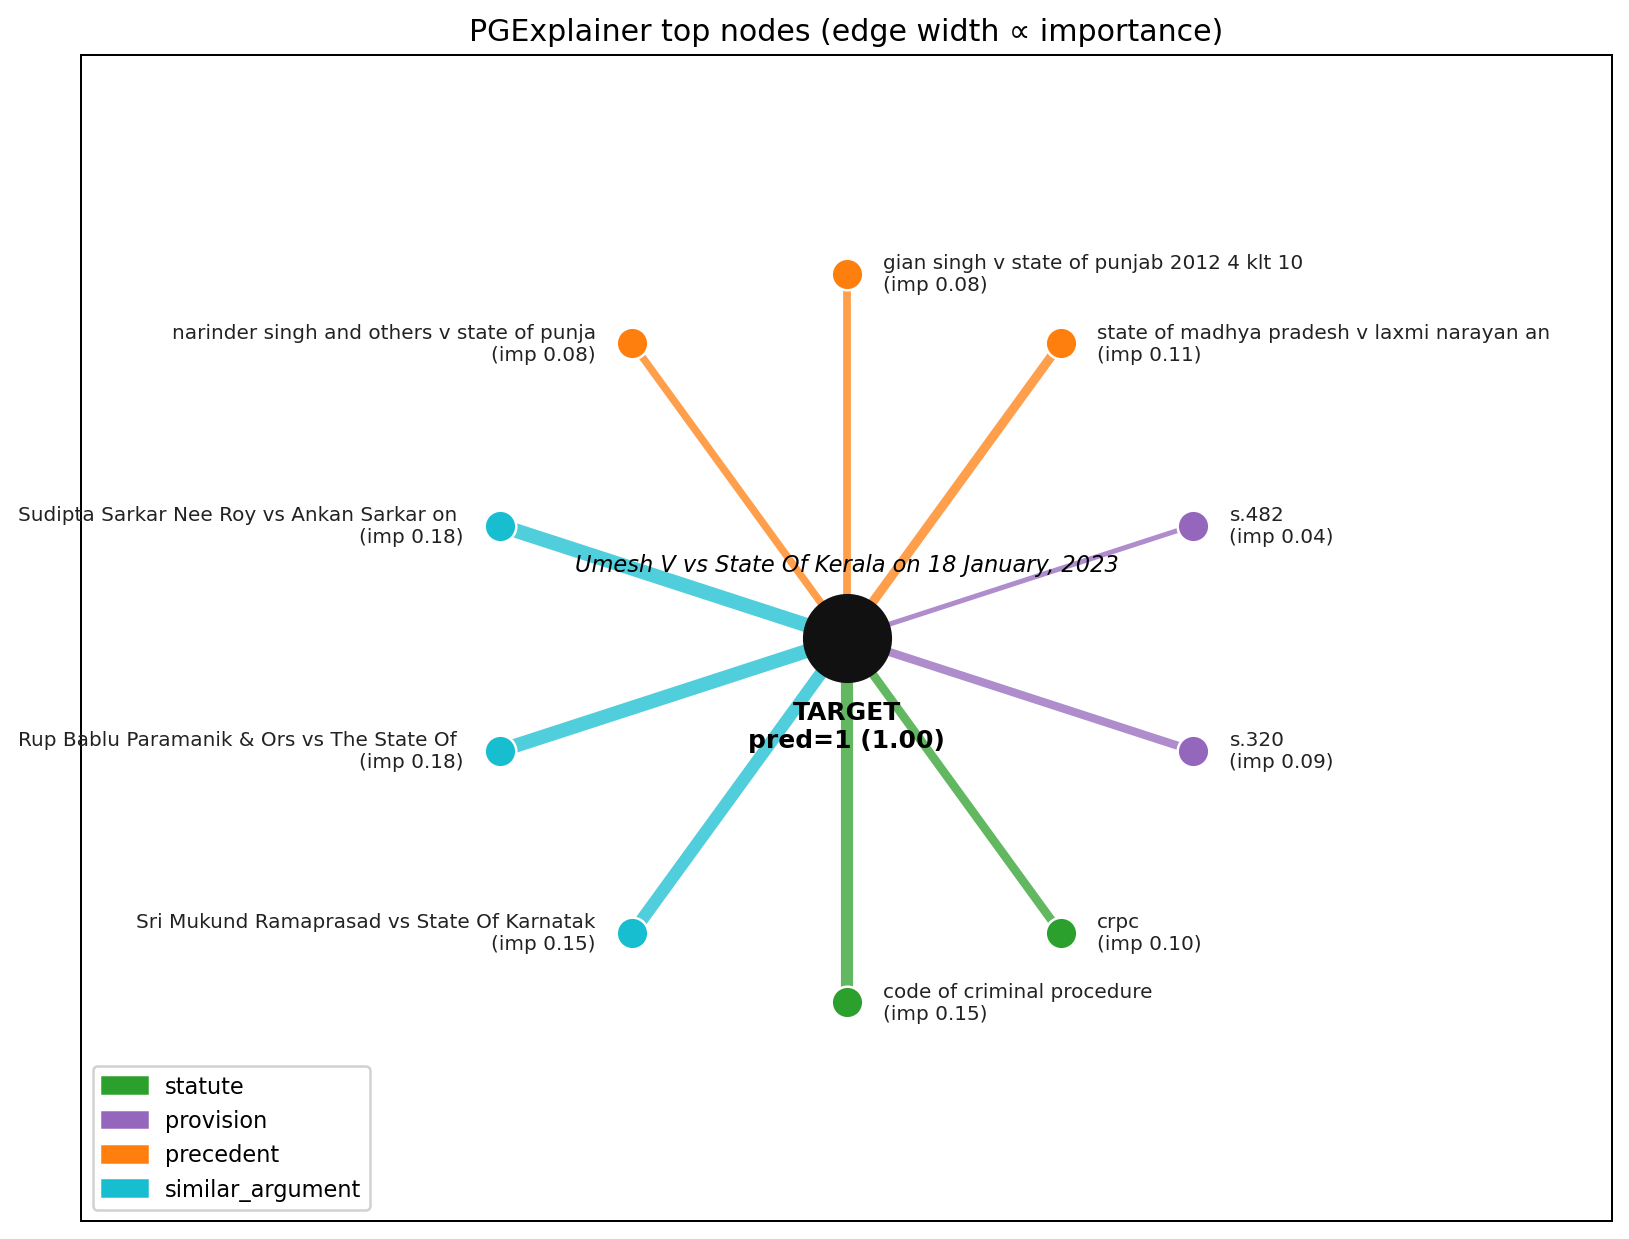
\includegraphics[width=\linewidth]{figures/explainability/wrong_13701_panel_b_subgraph.png}
  \end{minipage}
  \caption{Confidently-wrong case 13701 (\emph{Umesh V vs State of
  Kerala}, 2023).  The target sits inside a dense cluster of
  structurally near-identical Kerala cases filed on the same day,
  all of which are wins, so the retrieval-based explanation
  reinforces the (incorrect) predicted outcome.}
  \label{fig:case_wrong}
\end{figure}

The evidence subgraph and the retrieved neighbours are not
\emph{wrong} in any local sense: the cases \emph{are} structurally
very close to the target in the model's representation.  What the
failure reveals is that a small number of distinguishing facts ---
the specific factual configuration that led this particular court to
refuse relief --- do not survive the embedding transformation.  Read
alongside the aggregate statistic above, this is the structural
signature of confident error on this corpus.

\section{Summary}

The four-level pipeline presented in this chapter provides a
coherent interpretability story for the trained HGT.  At the
\emph{representation} level, a pre-GNN/post-GNN probe shows a
$+3.97$-point accuracy gain attributable to message passing, and
t-SNE confirms that the gain takes the form of within-domain outcome
reorganisation.  At the \emph{component} level, node-type zeroing,
per-relation attention, and SHAP all converge on the same story: the
\textsc{Case} node dominates, but argument nodes and the immediate
participants contribute measurable graph-local signal that a plain
text classifier cannot access.  At the \emph{error} level, residual
mistakes concentrate in doctrinally crowded cases, in the fraud and
sexual-offence buckets, and in the longest facts quintile --- all
structural properties of the data rather than of any specific model
configuration.  At the \emph{case} level, the \path{Graph_Analyser}
pipeline --- frozen inference, FAISS retrieval, heterogeneous
PGExplainer, and LLM translation --- produces grounded, legally
named explanations for individual predictions.

Crucially, the same pipeline exposes the model's \emph{confident}
failure mode.  For high-confidence predictions that are nevertheless
wrong, the top-$k$ retrieved neighbours overwhelmingly match the
predicted (incorrect) label rather than the true one.  This is the
sharpest single diagnostic the interpretability layer produces: a
confident error is not an isolated mistake but a case placed inside
the wrong outcome neighbourhood, whose explanation and whose
prediction reinforce each other.  Making that visible is what
distinguishes a post-hoc explainer from a calibration metric, and it
is the part of the pipeline with the clearest operational value for
deployment.
